% Options for packages loaded elsewhere
\PassOptionsToPackage{unicode}{hyperref}
\PassOptionsToPackage{hyphens}{url}
\PassOptionsToPackage{dvipsnames,svgnames,x11names}{xcolor}
%
\documentclass[
  letterpaper,
  DIV=11,
  numbers=noendperiod]{scrreport}

\usepackage{amsmath,amssymb}
\usepackage{lmodern}
\usepackage{iftex}
\ifPDFTeX
  \usepackage[T1]{fontenc}
  \usepackage[utf8]{inputenc}
  \usepackage{textcomp} % provide euro and other symbols
\else % if luatex or xetex
  \usepackage{unicode-math}
  \defaultfontfeatures{Scale=MatchLowercase}
  \defaultfontfeatures[\rmfamily]{Ligatures=TeX,Scale=1}
\fi
% Use upquote if available, for straight quotes in verbatim environments
\IfFileExists{upquote.sty}{\usepackage{upquote}}{}
\IfFileExists{microtype.sty}{% use microtype if available
  \usepackage[]{microtype}
  \UseMicrotypeSet[protrusion]{basicmath} % disable protrusion for tt fonts
}{}
\makeatletter
\@ifundefined{KOMAClassName}{% if non-KOMA class
  \IfFileExists{parskip.sty}{%
    \usepackage{parskip}
  }{% else
    \setlength{\parindent}{0pt}
    \setlength{\parskip}{6pt plus 2pt minus 1pt}}
}{% if KOMA class
  \KOMAoptions{parskip=half}}
\makeatother
\usepackage{xcolor}
\setlength{\emergencystretch}{3em} % prevent overfull lines
\setcounter{secnumdepth}{5}
% Make \paragraph and \subparagraph free-standing
\ifx\paragraph\undefined\else
  \let\oldparagraph\paragraph
  \renewcommand{\paragraph}[1]{\oldparagraph{#1}\mbox{}}
\fi
\ifx\subparagraph\undefined\else
  \let\oldsubparagraph\subparagraph
  \renewcommand{\subparagraph}[1]{\oldsubparagraph{#1}\mbox{}}
\fi

\usepackage{color}
\usepackage{fancyvrb}
\newcommand{\VerbBar}{|}
\newcommand{\VERB}{\Verb[commandchars=\\\{\}]}
\DefineVerbatimEnvironment{Highlighting}{Verbatim}{commandchars=\\\{\}}
% Add ',fontsize=\small' for more characters per line
\usepackage{framed}
\definecolor{shadecolor}{RGB}{241,243,245}
\newenvironment{Shaded}{\begin{snugshade}}{\end{snugshade}}
\newcommand{\AlertTok}[1]{\textcolor[rgb]{0.68,0.00,0.00}{#1}}
\newcommand{\AnnotationTok}[1]{\textcolor[rgb]{0.37,0.37,0.37}{#1}}
\newcommand{\AttributeTok}[1]{\textcolor[rgb]{0.40,0.45,0.13}{#1}}
\newcommand{\BaseNTok}[1]{\textcolor[rgb]{0.68,0.00,0.00}{#1}}
\newcommand{\BuiltInTok}[1]{\textcolor[rgb]{0.00,0.23,0.31}{#1}}
\newcommand{\CharTok}[1]{\textcolor[rgb]{0.13,0.47,0.30}{#1}}
\newcommand{\CommentTok}[1]{\textcolor[rgb]{0.37,0.37,0.37}{#1}}
\newcommand{\CommentVarTok}[1]{\textcolor[rgb]{0.37,0.37,0.37}{\textit{#1}}}
\newcommand{\ConstantTok}[1]{\textcolor[rgb]{0.56,0.35,0.01}{#1}}
\newcommand{\ControlFlowTok}[1]{\textcolor[rgb]{0.00,0.23,0.31}{#1}}
\newcommand{\DataTypeTok}[1]{\textcolor[rgb]{0.68,0.00,0.00}{#1}}
\newcommand{\DecValTok}[1]{\textcolor[rgb]{0.68,0.00,0.00}{#1}}
\newcommand{\DocumentationTok}[1]{\textcolor[rgb]{0.37,0.37,0.37}{\textit{#1}}}
\newcommand{\ErrorTok}[1]{\textcolor[rgb]{0.68,0.00,0.00}{#1}}
\newcommand{\ExtensionTok}[1]{\textcolor[rgb]{0.00,0.23,0.31}{#1}}
\newcommand{\FloatTok}[1]{\textcolor[rgb]{0.68,0.00,0.00}{#1}}
\newcommand{\FunctionTok}[1]{\textcolor[rgb]{0.28,0.35,0.67}{#1}}
\newcommand{\ImportTok}[1]{\textcolor[rgb]{0.00,0.46,0.62}{#1}}
\newcommand{\InformationTok}[1]{\textcolor[rgb]{0.37,0.37,0.37}{#1}}
\newcommand{\KeywordTok}[1]{\textcolor[rgb]{0.00,0.23,0.31}{#1}}
\newcommand{\NormalTok}[1]{\textcolor[rgb]{0.00,0.23,0.31}{#1}}
\newcommand{\OperatorTok}[1]{\textcolor[rgb]{0.37,0.37,0.37}{#1}}
\newcommand{\OtherTok}[1]{\textcolor[rgb]{0.00,0.23,0.31}{#1}}
\newcommand{\PreprocessorTok}[1]{\textcolor[rgb]{0.68,0.00,0.00}{#1}}
\newcommand{\RegionMarkerTok}[1]{\textcolor[rgb]{0.00,0.23,0.31}{#1}}
\newcommand{\SpecialCharTok}[1]{\textcolor[rgb]{0.37,0.37,0.37}{#1}}
\newcommand{\SpecialStringTok}[1]{\textcolor[rgb]{0.13,0.47,0.30}{#1}}
\newcommand{\StringTok}[1]{\textcolor[rgb]{0.13,0.47,0.30}{#1}}
\newcommand{\VariableTok}[1]{\textcolor[rgb]{0.07,0.07,0.07}{#1}}
\newcommand{\VerbatimStringTok}[1]{\textcolor[rgb]{0.13,0.47,0.30}{#1}}
\newcommand{\WarningTok}[1]{\textcolor[rgb]{0.37,0.37,0.37}{\textit{#1}}}

\providecommand{\tightlist}{%
  \setlength{\itemsep}{0pt}\setlength{\parskip}{0pt}}\usepackage{longtable,booktabs,array}
\usepackage{calc} % for calculating minipage widths
% Correct order of tables after \paragraph or \subparagraph
\usepackage{etoolbox}
\makeatletter
\patchcmd\longtable{\par}{\if@noskipsec\mbox{}\fi\par}{}{}
\makeatother
% Allow footnotes in longtable head/foot
\IfFileExists{footnotehyper.sty}{\usepackage{footnotehyper}}{\usepackage{footnote}}
\makesavenoteenv{longtable}
\usepackage{graphicx}
\makeatletter
\def\maxwidth{\ifdim\Gin@nat@width>\linewidth\linewidth\else\Gin@nat@width\fi}
\def\maxheight{\ifdim\Gin@nat@height>\textheight\textheight\else\Gin@nat@height\fi}
\makeatother
% Scale images if necessary, so that they will not overflow the page
% margins by default, and it is still possible to overwrite the defaults
% using explicit options in \includegraphics[width, height, ...]{}
\setkeys{Gin}{width=\maxwidth,height=\maxheight,keepaspectratio}
% Set default figure placement to htbp
\makeatletter
\def\fps@figure{htbp}
\makeatother

\usepackage{booktabs}
\usepackage{longtable}
\usepackage{array}
\usepackage{multirow}
\usepackage{wrapfig}
\usepackage{float}
\usepackage{colortbl}
\usepackage{pdflscape}
\usepackage{tabu}
\usepackage{threeparttable}
\usepackage{threeparttablex}
\usepackage[normalem]{ulem}
\usepackage{makecell}
\usepackage{xcolor}
\usepackage{caption}
\KOMAoption{captions}{tableheading}
\makeatletter
\makeatother
\makeatletter
\@ifpackageloaded{bookmark}{}{\usepackage{bookmark}}
\makeatother
\makeatletter
\@ifpackageloaded{caption}{}{\usepackage{caption}}
\AtBeginDocument{%
\ifdefined\contentsname
  \renewcommand*\contentsname{Table of contents}
\else
  \newcommand\contentsname{Table of contents}
\fi
\ifdefined\listfigurename
  \renewcommand*\listfigurename{List of Figures}
\else
  \newcommand\listfigurename{List of Figures}
\fi
\ifdefined\listtablename
  \renewcommand*\listtablename{List of Tables}
\else
  \newcommand\listtablename{List of Tables}
\fi
\ifdefined\figurename
  \renewcommand*\figurename{Figure}
\else
  \newcommand\figurename{Figure}
\fi
\ifdefined\tablename
  \renewcommand*\tablename{Table}
\else
  \newcommand\tablename{Table}
\fi
}
\@ifpackageloaded{float}{}{\usepackage{float}}
\floatstyle{ruled}
\@ifundefined{c@chapter}{\newfloat{codelisting}{h}{lop}}{\newfloat{codelisting}{h}{lop}[chapter]}
\floatname{codelisting}{Listing}
\newcommand*\listoflistings{\listof{codelisting}{List of Listings}}
\makeatother
\makeatletter
\@ifpackageloaded{caption}{}{\usepackage{caption}}
\@ifpackageloaded{subcaption}{}{\usepackage{subcaption}}
\makeatother
\makeatletter
\@ifpackageloaded{tcolorbox}{}{\usepackage[many]{tcolorbox}}
\makeatother
\makeatletter
\@ifundefined{shadecolor}{\definecolor{shadecolor}{rgb}{.97, .97, .97}}
\makeatother
\makeatletter
\makeatother
\ifLuaTeX
  \usepackage{selnolig}  % disable illegal ligatures
\fi
\IfFileExists{bookmark.sty}{\usepackage{bookmark}}{\usepackage{hyperref}}
\IfFileExists{xurl.sty}{\usepackage{xurl}}{} % add URL line breaks if available
\urlstyle{same} % disable monospaced font for URLs
\hypersetup{
  pdftitle={Methods (BST 232) Notes},
  pdfauthor={Christian Testa},
  colorlinks=true,
  linkcolor={blue},
  filecolor={Maroon},
  citecolor={Blue},
  urlcolor={Blue},
  pdfcreator={LaTeX via pandoc}}

\title{Methods (BST 232) Notes}
\author{Christian Testa}
\date{}

\begin{document}
\maketitle
\ifdefined\Shaded\renewenvironment{Shaded}{\begin{tcolorbox}[frame hidden, breakable, borderline west={3pt}{0pt}{shadecolor}, interior hidden, boxrule=0pt, enhanced, sharp corners]}{\end{tcolorbox}}\fi

\renewcommand*\contentsname{Table of contents}
{
\hypersetup{linkcolor=}
\setcounter{tocdepth}{2}
\tableofcontents
}
\bookmarksetup{startatroot}

\hypertarget{methods-bst-232-notes}{%
\chapter{Methods (BST 232) Notes}\label{methods-bst-232-notes}}

\bookmarksetup{startatroot}

\hypertarget{week-1}{%
\chapter{Week 1}\label{week-1}}

August 28 --- September 1, 2023

``By now you've probably figured out this is a class on linear models
and generalized linear models''

Office hours: Rachel: Fridays 4-5pm, in-person; Inte: Thursdays 3-4pm,
Zoom; Sal: Tuesdays 4-5pm, in-person

Lab time: Fridays: 2-3:30, usually Kresge LL6.

Use the discussion section of Canvas for random questions so everyone
has the same access to information.

We'll assume that students know random variables, hypothesis testing,
basic probability, etc.

Kutner et al's \emph{Applied Linear Statistical Models} book will be a
helpful reference for the first half of the class, while Agresti's
\emph{Categorical Data Analysis} will be more helpful for the second
half of the class.

\begin{figure}

{\centering \includegraphics[width=3.5in,height=\textheight]{week1/standalone_figures/scientific_process/scientific_process.svg}

}

\end{figure}

While it would be nice for statisticians to be more often than not
included in study design, it's quite usual that statisticians are often
sought out by their colleagues who bring them data that they want to
analyze. Hence our class will mostly take an interest in the indicated
section of the idealized scientific process, and moreover we'll assume
that we're often not in a randomized- controlled trial.

We'll focus on {associational studies}. While it's almost always the
case that when associational studies are performed that investigators
are actually interested in are {causal effects}. However, in this class
we'll tend not to talk about causal effects or ``causal'' -anything
because these days causal inference tends to refer to a specific set of
methods used in observational causal inference.

We'll be concerned quite substantively around confounding.

We'll talk about a lot of the methods that Ronald A. Fisher developed.
Already in the 1900s it was being observed that there was a strong
association between smoking and lung cancer. However, Fisher was a
smoker himself and posited that the association between lung cancer and
smoking could be explained away by some genetic or biological difference
between the smoking and non-smoking population (positing some genes that
caused people to desire to smoke).

\begin{figure}

{\centering \includegraphics[width=3.5in,height=\textheight]{week1/standalone_figures/confounding/smoking_confounding.svg}

}

\caption{Ronald Fisher's unsupported theory of genetics confounding the
smoking-lung cancer relationship}

\end{figure}

We're pretty sure that this was driven not by any substance matter
expertise, but rather by Fisher's love of smoking.

\hypertarget{hormone-replacement-therapy}{%
\section{Hormone Replacement
Therapy}\label{hormone-replacement-therapy}}

In the mid- to late- 20th century there were a ton of studies linking
hormone replacement therapy for older women to better cardiovascular
outcomes (lack of coronary heart disease).

However, thankfully due to the Heart and Estrogen/Progestin Study (HERS,
in the early 90s) we now know that a lot of those studies were not
controlling for socioeconomic status. It turns out that socioeconomic
status was highly associated with HRT usage, and associated at least in
the US with a lot of better health outcomes across the board.

It turned out that HRT when applied at certain times for some people can
actually be harmful --- but the point is the picture is much muddier
than was initially thought and recommendations were rolled back. Later
randomized studies were performed that produced reliable bodies of
evidence demonstrating either no effect or in some cases harmful
effects.

We'll use the baseline data from HERS (not so much interested in the HRT
treatment effect), but to investigate the research question:

\begin{quote}
How is systolic blood pressure related to age, independently of other
well-known cardiovascular risk factors? (Age, diabetes, smoking, etc.)
\end{quote}

\hypertarget{prediction-studies}{%
\section{Prediction Studies}\label{prediction-studies}}

Typically in prediction settings, there's no single exposure of
particular interest; mechanisms and confounding is treated as less of a
concern (if at all), and the main challenge is that we need to take care
to not {overfit} the data.

A major theme of this class will be that different tasks require
different analysis strategies and diffrent statistical tools.

\hypertarget{quantifying-uncertainty}{%
\section{Quantifying Uncertainty}\label{quantifying-uncertainty}}

Typically standard statistical models have nice theoretical properties
because years-and-years ago, we didn't have much data so people spent
their time studying theory instead of data. As a result, we have a lot
of nice theories about the uncertainty represented in statistical
models.

An example of the kind of uncertainty we might be interested in is shown
in this figure relating Alzheimer's disease rates and exposure to
PM\textsubscript{2.5}.

\begin{figure}

{\centering \includegraphics[width=4in,height=\textheight]{week1/standalone_figures/pm2.5/pm25.jpg}

}

\end{figure}

This figure is taken from the article
\href{https://www.thelancet.com/journals/lanplh/article/PIIS2542-5196(20)30227-8/fulltext}{\emph{Long-term
effects of PM2·5 on neurological disorders in the American Medicare
population: a longitudinal cohort study} by Shi et al, Lancet Planetary
Health (2020)}.

\hypertarget{why-learn-methods-before-study-design}{%
\section{Why Learn Methods Before Study
Design}\label{why-learn-methods-before-study-design}}

An interesting point made is that it's important to understand the
limitations, strengths of methods, what they can and can't do, and how
to use them before designing a study.

\hypertarget{recommended-reading}{%
\section{Recommended Reading}\label{recommended-reading}}

Kutner M, Nachtsheim C, Neter J, Li W. Applied Linear Statistical Model.
5th edition. chapters 1-3

Shmueli, G. (2010). To explain or to predict? \emph{Statistical
Science.}
\url{https://www.stat.berkeley.edu/~aldous/157/Papers/shmueli.pdf}

\bookmarksetup{startatroot}

\hypertarget{linear-regression}{%
\chapter{Linear Regression}\label{linear-regression}}

We will generally be intereseted in the relationship between an outcome
\(Y\) and \(p\) covariates or predictors denoted \((x_1, ..., x_p)\).

We generally say that a statistical model has a \emph{systematic}
component and a \emph{random} component.

We often hypothesize that the ``real'' relationship between our outcome
and predictors might be ``\emph{super-complex}''. Like cancer and
environmental exposures might have complex dependencies on genetics,
etc.. So sometimes instead of having a systematic component that
captures variables in their full complexity, we might prioritize
interpretability and we might be satisfied with an imperfect (but more
intuitive, simpler) model that might give us some intuition about
reality.

The random component may provide both a means to explain everything
uncaptured by our predictors, as well as ``real'' randomness. For
example, we might theorize that every time cells divide, there's some
small chance due to genetic drift that cells become metastatic and
cancerous which is just random (did a mutation happen that was harmful
in the right way in the right spot?).

\hypertarget{hers-study-sbp-in-post-menopausal-women}{%
\section{HERS Study: SBP in Post-Menopausal
Women}\label{hers-study-sbp-in-post-menopausal-women}}

In a clinical trial of hormone therapy for preventing heart attacks and
deaths among 2,763 post-menopausal women with existing coronary heart
disease:

\begin{itemize}
\tightlist
\item
  the outcome variable is systolic blood pressure
\item
  the data collected on covariates included age, diabetes diagnosis,
  smoking status, etc.
\item
  the research question was how is systolic blood pressure jointly
  related to age, statin use, and other risk factors in this cohort.
\end{itemize}

Reference: Vittinghoff et al., \emph{Regression methods in Biostatistics
2005}
\url{https://regression.ucsf.edu/regression-methods-biostatistics-linear-logistic-survival-and-repeated-measures-models}

\hypertarget{multiple-linear-regression-scalar-notation}{%
\section{Multiple Linear Regression: Scalar
Notation}\label{multiple-linear-regression-scalar-notation}}

We consider the model

\[Y_i = \beta_0 + \beta_1 x_{i1} + ... + \beta_p x_{ip} + \epsilon_i, \quad i = 1, ..., n.\]

\[\mathbb E(\epsilon_i) = 0, \, \underbrace{\text{Var}(\epsilon_i) = \sigma^2}_{\text{homoscedasticity assumption}}, \, \text{ and Cov}(\epsilon_i, \epsilon_j) = 0.\]

Typically we assume that the predictors \(x_i\) are fixed and measured
without error.

We require that \(p < n\).

TJ notes that \(\text{Cov}(\epsilon_i, \epsilon_j) = 0\) doesn't imply
independence. This is the assumption we're making for the time-being,
but independence will be implied after we later assume that the errors
are normally distributed.

Roman asks if we need a conditional mean zero assumption --- i.e.,
\(\mathbb E(\epsilon | x) = 0\)? Rachel notes that \(\epsilon\) and
\(x\) are assumed to be independent, so
\(\mathbb E(\epsilon | x) = \epsilon\). We will make stronger
assumptions later, but we aren't introducing those yet.

By taking the expected value of both sides, we can equivalently write
that

\[\mathbb E(Y_i) = \beta_0 + \beta_1 x_{i1} + ... + \beta_p x_{ip}.\]

The parameters \(\beta_j\) for \(j = 1, ..., p\) represent the change in
the expected value \(\mathbb E(Y_i)\) per unit change in \(x_j\) holding
the remaining predictors \(x_k \, (k \neq j)\) constant.

One can see this by observing:

\[ \mathbb E(Y_i | x_{i1} = x^* + 1) = \beta_0 + \beta_1 (x^* + 1) + ...\]
\[ \mathbb E(Y_i | x_{i1} = x^*) = \beta_0 + \beta_1 x^* + ...\]
\[ \mathbb E(Y_i | x_{i1} = x^* + 1) - \mathbb E(Y_i | x_{i1} = x^*) = \beta_1.\]

We most often interested in testing whether \(\beta_j = 0\), interpreted
as a test of whether there's an association between \(x_j\) and \(Y\).

\hypertarget{vector-notation}{%
\section{Vector Notation}\label{vector-notation}}

We can write this model more succinctly by writing:

\[ Y_i = x_i' \beta + \epsilon_i, \quad i = 1, ..., n,\]

where \(x_i = (1, x_{i1}, ..., x_{ip})',\) and
\(\beta = (\beta_0, \beta_1, ..., \beta_p)'\),
\(\mathbb E(\epsilon_i) = 0\), \(\text{Var}(\epsilon_i) = \sigma^2\),
and \(\text{Cov}(\epsilon_i, \epsilon_j) = 0\).

\hypertarget{examples}{%
\section{Examples}\label{examples}}

\begin{Shaded}
\begin{Highlighting}[]
\FunctionTok{library}\NormalTok{(here)}
\end{Highlighting}
\end{Shaded}

\begin{verbatim}
here() starts at /Users/cht180/Documents/2023/BST232 Methods Quarto
\end{verbatim}

\begin{Shaded}
\begin{Highlighting}[]
\FunctionTok{library}\NormalTok{(tidyverse)}
\end{Highlighting}
\end{Shaded}

\begin{verbatim}
-- Attaching core tidyverse packages ------------------------ tidyverse 2.0.0 --
v dplyr     1.1.2     v readr     2.1.4
v forcats   1.0.0     v stringr   1.5.0
v ggplot2   3.4.2     v tibble    3.2.1
v lubridate 1.9.2     v tidyr     1.3.0
v purrr     1.0.1     
\end{verbatim}

\begin{verbatim}
-- Conflicts ------------------------------------------ tidyverse_conflicts() --
x dplyr::filter() masks stats::filter()
x dplyr::lag()    masks stats::lag()
i Use the conflicted package (<http://conflicted.r-lib.org/>) to force all conflicts to become errors
\end{verbatim}

\begin{Shaded}
\begin{Highlighting}[]
\NormalTok{hers }\OtherTok{\textless{}{-}}\NormalTok{ readr}\SpecialCharTok{::}\FunctionTok{read\_csv}\NormalTok{(}\FunctionTok{here}\NormalTok{(}\StringTok{"data/hers.csv"}\NormalTok{))}
\end{Highlighting}
\end{Shaded}

\begin{verbatim}
Rows: 2763 Columns: 40
-- Column specification --------------------------------------------------------
Delimiter: ","
chr (16): HT, raceth, nonwhite, smoking, drinkany, exercise, physact, globra...
dbl (24): age, medcond, weight, BMI, waist, WHR, glucose, weight1, BMI1, wai...

i Use `spec()` to retrieve the full column specification for this data.
i Specify the column types or set `show_col_types = FALSE` to quiet this message.
\end{verbatim}

\begin{Shaded}
\begin{Highlighting}[]
\NormalTok{plt1 }\OtherTok{\textless{}{-}} \FunctionTok{ggplot}\NormalTok{(hers }\SpecialCharTok{\%\textgreater{}\%}\NormalTok{ dplyr}\SpecialCharTok{::}\FunctionTok{sample\_frac}\NormalTok{(.}\DecValTok{1}\NormalTok{), }\FunctionTok{aes}\NormalTok{(}\AttributeTok{x =}\NormalTok{ age, }\AttributeTok{y =}\NormalTok{ SBP)) }\SpecialCharTok{+} 
  \FunctionTok{geom\_point}\NormalTok{() }\SpecialCharTok{+} 
  \FunctionTok{theme\_bw}\NormalTok{() }\SpecialCharTok{+} 
  \FunctionTok{ggtitle}\NormalTok{(}\StringTok{"Scatterplot of a 10\% sample of our data"}\NormalTok{) }
\NormalTok{plt1 }
\end{Highlighting}
\end{Shaded}

\begin{figure}[H]

{\centering \includegraphics{week1/week1_files/figure-pdf/unnamed-chunk-4-1.pdf}

}

\end{figure}

\begin{Shaded}
\begin{Highlighting}[]
\NormalTok{plt2 }\OtherTok{\textless{}{-}}\NormalTok{ plt1 }\SpecialCharTok{+} 
  \FunctionTok{stat\_summary\_bin}\NormalTok{(}\AttributeTok{bins =} \DecValTok{10}\NormalTok{, }\AttributeTok{breaks =} \FunctionTok{quantile}\NormalTok{(hers}\SpecialCharTok{$}\NormalTok{age, }\FunctionTok{seq}\NormalTok{(}\DecValTok{0}\NormalTok{,}\DecValTok{1}\NormalTok{, }\FloatTok{0.1}\NormalTok{)), }\AttributeTok{geom =} \StringTok{\textquotesingle{}line\textquotesingle{}}\NormalTok{, }\AttributeTok{fun =}\NormalTok{ mean, }\AttributeTok{color =} \StringTok{\textquotesingle{}cadetblue\textquotesingle{}}\NormalTok{, }\AttributeTok{size =} \FloatTok{1.5}\NormalTok{) }\SpecialCharTok{+} 
  \FunctionTok{stat\_summary\_bin}\NormalTok{(}\AttributeTok{bins =} \DecValTok{10}\NormalTok{, }\AttributeTok{breaks =} \FunctionTok{quantile}\NormalTok{(hers}\SpecialCharTok{$}\NormalTok{age, }\FunctionTok{seq}\NormalTok{(}\DecValTok{0}\NormalTok{,}\DecValTok{1}\NormalTok{, }\FloatTok{0.1}\NormalTok{)), }\AttributeTok{geom =} \StringTok{\textquotesingle{}point\textquotesingle{}}\NormalTok{, }\AttributeTok{shape =} \DecValTok{23}\NormalTok{, }\AttributeTok{fun =}\NormalTok{ mean, }\AttributeTok{color =} \StringTok{\textquotesingle{}black\textquotesingle{}}\NormalTok{, }\AttributeTok{size =} \FloatTok{3.5}\NormalTok{, }\AttributeTok{fill =} \StringTok{\textquotesingle{}white\textquotesingle{}}\NormalTok{) }\SpecialCharTok{+} 
  \FunctionTok{ggtitle}\NormalTok{(}\StringTok{"Now with overlain means for decile groups by age"}\NormalTok{)}
\end{Highlighting}
\end{Shaded}

\begin{verbatim}
Warning: Using `size` aesthetic for lines was deprecated in ggplot2 3.4.0.
i Please use `linewidth` instead.
\end{verbatim}

\begin{Shaded}
\begin{Highlighting}[]
\NormalTok{plt2 }
\end{Highlighting}
\end{Shaded}

\begin{figure}[H]

{\centering \includegraphics{week1/week1_files/figure-pdf/unnamed-chunk-4-2.pdf}

}

\end{figure}

\begin{Shaded}
\begin{Highlighting}[]
\NormalTok{plt3 }\OtherTok{\textless{}{-}} 
\NormalTok{  plt2 }\SpecialCharTok{+} 
  \FunctionTok{geom\_smooth}\NormalTok{(}\AttributeTok{method =} \StringTok{\textquotesingle{}lm\textquotesingle{}}\NormalTok{, }\AttributeTok{se =} \ConstantTok{FALSE}\NormalTok{) }\SpecialCharTok{+} 
  \FunctionTok{ggtitle}\NormalTok{(}\StringTok{"Now with a linear model"}\NormalTok{) }
\NormalTok{plt3 }
\end{Highlighting}
\end{Shaded}

\begin{verbatim}
`geom_smooth()` using formula = 'y ~ x'
\end{verbatim}

\begin{figure}[H]

{\centering \includegraphics{week1/week1_files/figure-pdf/unnamed-chunk-4-3.pdf}

}

\end{figure}

\begin{Shaded}
\begin{Highlighting}[]
\NormalTok{lm.sbp.age }\OtherTok{\textless{}{-}} \FunctionTok{lm}\NormalTok{(SBP }\SpecialCharTok{\textasciitilde{}}\NormalTok{ age, }\AttributeTok{data =}\NormalTok{ hers)}
\NormalTok{jtools}\SpecialCharTok{::}\FunctionTok{summ}\NormalTok{(lm.sbp.age)}
\end{Highlighting}
\end{Shaded}

\begin{table}[!h]
\centering
\begin{tabular}{lr}
\toprule
\cellcolor{gray!6}{Observations} & \cellcolor{gray!6}{2763}\\
Dependent variable & SBP\\
\cellcolor{gray!6}{Type} & \cellcolor{gray!6}{OLS linear regression}\\
\bottomrule
\end{tabular}
\end{table} \begin{table}[!h]
\centering
\begin{tabular}{lr}
\toprule
\cellcolor{gray!6}{F(1,2761)} & \cellcolor{gray!6}{77.21}\\
R² & 0.03\\
\cellcolor{gray!6}{Adj. R²} & \cellcolor{gray!6}{0.03}\\
\bottomrule
\end{tabular}
\end{table} \begin{table}[!h]
\centering
\begin{threeparttable}
\begin{tabular}{lrrrr}
\toprule
  & Est. & S.E. & t val. & p\\
\midrule
\cellcolor{gray!6}{(Intercept)} & \cellcolor{gray!6}{103.63} & \cellcolor{gray!6}{3.60} & \cellcolor{gray!6}{28.82} & \cellcolor{gray!6}{0.00}\\
age & 0.47 & 0.05 & 8.79 & 0.00\\
\bottomrule
\end{tabular}
\begin{tablenotes}
\item Standard errors: OLS
\end{tablenotes}
\end{threeparttable}
\end{table}

So now we would say that
\(\hat{\mathbb E}(SBP_i) = 103.63 + 103.63 Age_i\). Though, the
intercept is kind of useless since our model doesn't have any
observations for systolic blood pressure for age 0 infants. We might
want to fit an age centered model.

\begin{Shaded}
\begin{Highlighting}[]
\NormalTok{lm.sbp.agec }\OtherTok{\textless{}{-}} \FunctionTok{lm}\NormalTok{(SBP }\SpecialCharTok{\textasciitilde{}} \FunctionTok{I}\NormalTok{(age }\SpecialCharTok{{-}} \FunctionTok{mean}\NormalTok{(age)), }\AttributeTok{data =}\NormalTok{ hers)}
\NormalTok{jtools}\SpecialCharTok{::}\FunctionTok{summ}\NormalTok{(lm.sbp.agec)}
\end{Highlighting}
\end{Shaded}

\begin{table}[!h]
\centering
\begin{tabular}{lr}
\toprule
\cellcolor{gray!6}{Observations} & \cellcolor{gray!6}{2763}\\
Dependent variable & SBP\\
\cellcolor{gray!6}{Type} & \cellcolor{gray!6}{OLS linear regression}\\
\bottomrule
\end{tabular}
\end{table} \begin{table}[!h]
\centering
\begin{tabular}{lr}
\toprule
\cellcolor{gray!6}{F(1,2761)} & \cellcolor{gray!6}{77.21}\\
R² & 0.03\\
\cellcolor{gray!6}{Adj. R²} & \cellcolor{gray!6}{0.03}\\
\bottomrule
\end{tabular}
\end{table} \begin{table}[!h]
\centering
\begin{threeparttable}
\begin{tabular}{lrrrr}
\toprule
  & Est. & S.E. & t val. & p\\
\midrule
\cellcolor{gray!6}{(Intercept)} & \cellcolor{gray!6}{135.07} & \cellcolor{gray!6}{0.36} & \cellcolor{gray!6}{378.24} & \cellcolor{gray!6}{0.00}\\
I(age - mean(age)) & 0.47 & 0.05 & 8.79 & 0.00\\
\bottomrule
\end{tabular}
\begin{tablenotes}
\item Standard errors: OLS
\end{tablenotes}
\end{threeparttable}
\end{table}

In which case we'd say that
\(\hat{\mathbb E}(SBP_i) = 135.07 + 135.07 Age_i\).

\hypertarget{multiple-linear-regression}{%
\section{Multiple Linear Regression}\label{multiple-linear-regression}}

\begin{Shaded}
\begin{Highlighting}[]
\CommentTok{\# fitting a p=2 model}
\NormalTok{lm.sbp.age.weight }\OtherTok{\textless{}{-}} \FunctionTok{lm}\NormalTok{(SBP }\SpecialCharTok{\textasciitilde{}}\NormalTok{ age }\SpecialCharTok{+}\NormalTok{ weight, }\AttributeTok{data =}\NormalTok{ hers)}
\NormalTok{x }\OtherTok{\textless{}{-}}\NormalTok{ y }\OtherTok{\textless{}{-}} \FunctionTok{seq}\NormalTok{(}\DecValTok{0}\NormalTok{, }\DecValTok{100}\NormalTok{, }\AttributeTok{length=} \DecValTok{30}\NormalTok{)}
\NormalTok{f }\OtherTok{\textless{}{-}} \ControlFlowTok{function}\NormalTok{(x,y)\{ z }\OtherTok{\textless{}{-}}\NormalTok{ x}\SpecialCharTok{*}\FunctionTok{coef}\NormalTok{(lm.sbp.age.weight)[}\DecValTok{2}\NormalTok{] }\SpecialCharTok{+}\NormalTok{ y}\SpecialCharTok{*}\FunctionTok{coef}\NormalTok{(lm.sbp.age.weight)[}\DecValTok{3}\NormalTok{] }\SpecialCharTok{+} \FunctionTok{coef}\NormalTok{(lm.sbp.age.weight)[}\DecValTok{1}\NormalTok{] \}}
\NormalTok{z }\OtherTok{\textless{}{-}} \FunctionTok{outer}\NormalTok{(x,y,f)}
\FunctionTok{persp}\NormalTok{(x, y, z, }\AttributeTok{theta =} \DecValTok{30}\NormalTok{, }\AttributeTok{phi =} \DecValTok{30}\NormalTok{, }\AttributeTok{expand =} \FloatTok{0.5}\NormalTok{, }\AttributeTok{col =} \StringTok{"lightblue"}\NormalTok{, }\AttributeTok{xlab =} \StringTok{"age"}\NormalTok{, }\AttributeTok{ylab =} \StringTok{"weight"}\NormalTok{, }\AttributeTok{zlab =} \StringTok{"expected SBP"}\NormalTok{, }\AttributeTok{ticktype =} \StringTok{\textquotesingle{}detailed\textquotesingle{}}\NormalTok{, }\AttributeTok{nticks =} \DecValTok{4}\NormalTok{)}
\end{Highlighting}
\end{Shaded}

\begin{figure}[H]

{\centering \includegraphics{week1/week1_files/figure-pdf/unnamed-chunk-7-1.pdf}

}

\end{figure}

\hypertarget{indicator-dummy-variables}{%
\section{Indicator / Dummy Variables}\label{indicator-dummy-variables}}

We might be interested in modeling categorical variables as well. To do
so, we would include dummy variables.

If a categorical variable has \(K\) levels, then we'll need to compute
\(K-1\) dummy variables where the omitted variable is called the
``reference level''.

\begin{Shaded}
\begin{Highlighting}[]
\FunctionTok{unique}\NormalTok{(hers}\SpecialCharTok{$}\NormalTok{physact)}
\end{Highlighting}
\end{Shaded}

\begin{verbatim}
[1] "much more active"     "much less active"     "about as active"     
[4] "somewhat less active" "somewhat more active"
\end{verbatim}

\begin{Shaded}
\begin{Highlighting}[]
\NormalTok{hers}\SpecialCharTok{$}\NormalTok{physact }\OtherTok{\textless{}{-}} \FunctionTok{as.factor}\NormalTok{(hers}\SpecialCharTok{$}\NormalTok{physact) }
\CommentTok{\# the reference category will be "much more active" since it\textquotesingle{}s the }
\CommentTok{\# first factor level — }
\CommentTok{\# if we wanted to change it, we could run: }
\CommentTok{\# hers$raceth \textless{}{-} relevel(hers$raceth, "much less active") }
\CommentTok{\# for example. }
\NormalTok{lm.sbp.physact }\OtherTok{\textless{}{-}} \FunctionTok{lm}\NormalTok{(SBP }\SpecialCharTok{\textasciitilde{}}\NormalTok{ physact, }\AttributeTok{data =}\NormalTok{ hers)}
\FunctionTok{head}\NormalTok{(}\FunctionTok{model.matrix}\NormalTok{(lm.sbp.physact))}
\end{Highlighting}
\end{Shaded}

\begin{verbatim}
  (Intercept) physactmuch less active physactmuch more active
1           1                       0                       1
2           1                       1                       0
3           1                       0                       0
4           1                       1                       0
5           1                       0                       0
6           1                       0                       0
  physactsomewhat less active physactsomewhat more active
1                           0                           0
2                           0                           0
3                           0                           0
4                           0                           0
5                           1                           0
6                           0                           0
\end{verbatim}

\begin{Shaded}
\begin{Highlighting}[]
\NormalTok{jtools}\SpecialCharTok{::}\FunctionTok{summ}\NormalTok{(lm.sbp.physact)}
\end{Highlighting}
\end{Shaded}

\begin{table}[!h]
\centering
\begin{tabular}{lr}
\toprule
\cellcolor{gray!6}{Observations} & \cellcolor{gray!6}{2763}\\
Dependent variable & SBP\\
\cellcolor{gray!6}{Type} & \cellcolor{gray!6}{OLS linear regression}\\
\bottomrule
\end{tabular}
\end{table} \begin{table}[!h]
\centering
\begin{tabular}{lr}
\toprule
\cellcolor{gray!6}{F(4,2758)} & \cellcolor{gray!6}{0.48}\\
R² & 0.00\\
\cellcolor{gray!6}{Adj. R²} & \cellcolor{gray!6}{-0.00}\\
\bottomrule
\end{tabular}
\end{table} \begin{table}[!h]
\centering
\begin{threeparttable}
\begin{tabular}{lrrrr}
\toprule
  & Est. & S.E. & t val. & p\\
\midrule
\cellcolor{gray!6}{(Intercept)} & \cellcolor{gray!6}{135.00} & \cellcolor{gray!6}{0.63} & \cellcolor{gray!6}{215.01} & \cellcolor{gray!6}{0.00}\\
physactmuch less active & 0.07 & 1.49 & 0.05 & 0.96\\
\cellcolor{gray!6}{physactmuch more active} & \cellcolor{gray!6}{-0.90} & \cellcolor{gray!6}{1.26} & \cellcolor{gray!6}{-0.72} & \cellcolor{gray!6}{0.47}\\
physactsomewhat less active & 0.96 & 1.06 & 0.91 & 0.36\\
\cellcolor{gray!6}{physactsomewhat more active} & \cellcolor{gray!6}{-0.05} & \cellcolor{gray!6}{0.91} & \cellcolor{gray!6}{-0.05} & \cellcolor{gray!6}{0.96}\\
\bottomrule
\end{tabular}
\begin{tablenotes}
\item Standard errors: OLS
\end{tablenotes}
\end{threeparttable}
\end{table}

In machine learning this is called
\href{https://en.wikipedia.org/wiki/One-hot}{``one-hot'' encoding}.

\hypertarget{polynomial-regressions}{%
\section{Polynomial Regressions}\label{polynomial-regressions}}

\begin{Shaded}
\begin{Highlighting}[]
\NormalTok{lm.sbp.agepolynomial }\OtherTok{\textless{}{-}} \FunctionTok{lm}\NormalTok{(SBP }\SpecialCharTok{\textasciitilde{}} \FunctionTok{poly}\NormalTok{(age), }\AttributeTok{data =}\NormalTok{ hers)}

\CommentTok{\# we could plug in coef(lm.sbp.agepolynomial)[1] through }
\CommentTok{\# coef(lm.sbp.agepolynomial)[4] into the following equation, }
\CommentTok{\# but it\textquotesingle{}s kind of boring — instead here\textquotesingle{}s a more fun }
\CommentTok{\# looking cubic polynomial we could imagine being the result of}
\CommentTok{\# a polynomial regression:}
\FunctionTok{curve}\NormalTok{(}\DecValTok{1} \SpecialCharTok{{-}} \FloatTok{2.8}\SpecialCharTok{*}\NormalTok{x }\SpecialCharTok{+} \DecValTok{4}\SpecialCharTok{*}\NormalTok{(x}\SpecialCharTok{\^{}}\DecValTok{2}\NormalTok{) }\SpecialCharTok{{-}}\NormalTok{ .}\DecValTok{65}\SpecialCharTok{*}\NormalTok{(x}\SpecialCharTok{\^{}}\DecValTok{3}\NormalTok{), }\AttributeTok{from =} \DecValTok{0}\NormalTok{, }\AttributeTok{to =} \DecValTok{5}\NormalTok{,}
      \AttributeTok{xlab =} \FunctionTok{expression}\NormalTok{(x[}\DecValTok{1}\NormalTok{]),}
      \AttributeTok{ylab =} \StringTok{"E(Y)"}\NormalTok{)}
\end{Highlighting}
\end{Shaded}

\begin{figure}[H]

{\centering \includegraphics{week1/week1_files/figure-pdf/unnamed-chunk-9-1.pdf}

}

\end{figure}

It's worth emphasizing that usually we prefer splines or generalized
additive models to polynomial regression these days since polynomial
regression can act strangely.

\hypertarget{marginal-associations}{%
\section{Marginal Associations}\label{marginal-associations}}

If we have one binary predictor \(x_1\) and one continuous \(x_2\), we
might be interested in the \emph{marginal association} between \(Y\) and
\(x_2\). This would look like a model fit with
\texttt{lm(Y\ \textasciitilde{}\ x2)} and \(x_1\) is not included.

\hypertarget{conditional-association}{%
\section{Conditional Association}\label{conditional-association}}

We might also want to fit models that include \(x_1\), so those could be
fit with \texttt{lm(Y\ \textasciitilde{}\ x1\ +\ x2)} and this would
include an effect for \(x_2\) (one effect, not multiple) that is applied
while also considering an effect for \(x1\).

\bookmarksetup{startatroot}

\hypertarget{week-2}{%
\chapter{Week 2}\label{week-2}}

Equivalent forms of the canonical linear model:

Assuming \(\mathbb E[\epsilon_i] = 0\),
\(\text{Var}(\epsilon_i) = \sigma^2\),
\(\text{Cov}(\epsilon_i, \epsilon_i') = 0\).

Scalar notation:
\[ Y_i = \beta_0 + \beta_1 x_{i1} + ... + \beta_p x_{ip} + \epsilon_i\]

Vector notation

\[ Y_i = x_i' \beta + \epsilon_i\]

Expectation representations

\[\mathbb E(Y_i) = \beta_0 + \beta_1 x_{i1} + ... + \beta_p x_{ip}\]
\[\mathbb E(Y_i) = x_i' \beta\]

Parameter interpretation: the \(\beta\) values represent the change in
expected value per unit change in \(x\) holding the remaining predictors
constant.

Best practices:

\begin{itemize}
\tightlist
\item
  Always include an intercept, even if it's not interpretable or of
  substantive interest.
\item
  For \(K\)-category predictors, include \(K-1\) indicators in
  regression (leads to ANOVA-like situations).
\item
  If relationships are suspected to be nonlinear, can include polynomial
  or other nonlinear terms.
\end{itemize}

\hypertarget{confounding}{%
\section{Confounding}\label{confounding}}

Given an outcome \(Y\) and two covariates \(x1\) and \(x2\), should we
include \(x1\) in the model?

Suppose we didn't see the data generation process:

\begin{Shaded}
\begin{Highlighting}[]
\NormalTok{x2 }\OtherTok{\textless{}{-}} \FunctionTok{rnorm}\NormalTok{(}\AttributeTok{n =} \DecValTok{100}\NormalTok{, }\AttributeTok{mean =} \FloatTok{3.25}\NormalTok{, }\AttributeTok{sd =}\NormalTok{ .}\DecValTok{15}\NormalTok{)}
\NormalTok{Y }\OtherTok{\textless{}{-}}\NormalTok{ x2}\SpecialCharTok{*}\FloatTok{1.5} \SpecialCharTok{+} \FunctionTok{rnorm}\NormalTok{(}\AttributeTok{n =} \DecValTok{100}\NormalTok{)}
\NormalTok{x1 }\OtherTok{\textless{}{-}}\NormalTok{ (x2 }\SpecialCharTok{+}\NormalTok{ Y }\SpecialCharTok{\textgreater{}} \DecValTok{8}\NormalTok{)}
\end{Highlighting}
\end{Shaded}

But we could see marginal associations:

\begin{Shaded}
\begin{Highlighting}[]
\FunctionTok{library}\NormalTok{(tidyverse)}
\end{Highlighting}
\end{Shaded}

\begin{verbatim}
-- Attaching core tidyverse packages ------------------------ tidyverse 2.0.0 --
v dplyr     1.1.2     v readr     2.1.4
v forcats   1.0.0     v stringr   1.5.0
v ggplot2   3.4.2     v tibble    3.2.1
v lubridate 1.9.2     v tidyr     1.3.0
v purrr     1.0.1     
-- Conflicts ------------------------------------------ tidyverse_conflicts() --
x dplyr::filter() masks stats::filter()
x dplyr::lag()    masks stats::lag()
i Use the conflicted package (<http://conflicted.r-lib.org/>) to force all conflicts to become errors
\end{verbatim}

\begin{Shaded}
\begin{Highlighting}[]
\FunctionTok{ggplot}\NormalTok{(}\FunctionTok{data.frame}\NormalTok{(), }\FunctionTok{aes}\NormalTok{(}\AttributeTok{x =}\NormalTok{ x2, }\AttributeTok{y =}\NormalTok{ Y, }\AttributeTok{color =}\NormalTok{ x1, }\AttributeTok{shape =}\NormalTok{ x1)) }\SpecialCharTok{+} 
  \FunctionTok{geom\_point}\NormalTok{() }\SpecialCharTok{+} 
  \FunctionTok{theme\_bw}\NormalTok{() }\SpecialCharTok{+} 
  \FunctionTok{theme}\NormalTok{(}\AttributeTok{legend.position =} \StringTok{\textquotesingle{}bottom\textquotesingle{}}\NormalTok{) }\SpecialCharTok{+} 
  \FunctionTok{ggtitle}\NormalTok{(}\FunctionTok{expression}\NormalTok{(}\FunctionTok{paste}\NormalTok{(x[}\DecValTok{1}\NormalTok{], }\StringTok{" confounds the relationship between "}\NormalTok{,}
\NormalTok{                           x[}\DecValTok{2}\NormalTok{], }\StringTok{" and "}\NormalTok{, Y)))}
\end{Highlighting}
\end{Shaded}

\begin{figure}[H]

{\centering 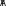
\includegraphics{week2/week2_files/figure-pdf/unnamed-chunk-2-1.pdf}

}

\end{figure}

Which would show us that \(x_1\) is associated with both \(x_2\) and
\(Y\).

Fitting a model with both \(x_1\) and \(x_2\), we would call the
prediction of \(Y\) given \(x_2\) the conditional association between
\(x_2\) conditional on (or within levels of) \(x_1\).

\begin{Shaded}
\begin{Highlighting}[]
\CommentTok{\# observe that the association flips}
\NormalTok{jtools}\SpecialCharTok{::}\FunctionTok{summ}\NormalTok{(}\FunctionTok{lm}\NormalTok{(Y }\SpecialCharTok{\textasciitilde{}}\NormalTok{ x2))}
\end{Highlighting}
\end{Shaded}

\begin{table}[!h]
\centering
\begin{tabular}{lr}
\toprule
\cellcolor{gray!6}{Observations} & \cellcolor{gray!6}{100}\\
Dependent variable & Y\\
\cellcolor{gray!6}{Type} & \cellcolor{gray!6}{OLS linear regression}\\
\bottomrule
\end{tabular}
\end{table} \begin{table}[!h]
\centering
\begin{tabular}{lr}
\toprule
\cellcolor{gray!6}{F(1,98)} & \cellcolor{gray!6}{1.30}\\
R² & 0.01\\
\cellcolor{gray!6}{Adj. R²} & \cellcolor{gray!6}{0.00}\\
\bottomrule
\end{tabular}
\end{table} \begin{table}[!h]
\centering
\begin{threeparttable}
\begin{tabular}{lrrrr}
\toprule
  & Est. & S.E. & t val. & p\\
\midrule
\cellcolor{gray!6}{(Intercept)} & \cellcolor{gray!6}{2.46} & \cellcolor{gray!6}{2.13} & \cellcolor{gray!6}{1.16} & \cellcolor{gray!6}{0.25}\\
x2 & 0.74 & 0.65 & 1.14 & 0.26\\
\bottomrule
\end{tabular}
\begin{tablenotes}
\item Standard errors: OLS
\end{tablenotes}
\end{threeparttable}
\end{table}

\begin{Shaded}
\begin{Highlighting}[]
\NormalTok{jtools}\SpecialCharTok{::}\FunctionTok{summ}\NormalTok{(}\FunctionTok{lm}\NormalTok{(Y }\SpecialCharTok{\textasciitilde{}}\NormalTok{ x1 }\SpecialCharTok{+}\NormalTok{ x2))}
\end{Highlighting}
\end{Shaded}

\begin{table}[!h]
\centering
\begin{tabular}{lr}
\toprule
\cellcolor{gray!6}{Observations} & \cellcolor{gray!6}{100}\\
Dependent variable & Y\\
\cellcolor{gray!6}{Type} & \cellcolor{gray!6}{OLS linear regression}\\
\bottomrule
\end{tabular}
\end{table} \begin{table}[!h]
\centering
\begin{tabular}{lr}
\toprule
\cellcolor{gray!6}{F(2,97)} & \cellcolor{gray!6}{89.79}\\
R² & 0.65\\
\cellcolor{gray!6}{Adj. R²} & \cellcolor{gray!6}{0.64}\\
\bottomrule
\end{tabular}
\end{table} \begin{table}[!h]
\centering
\begin{threeparttable}
\begin{tabular}{lrrrr}
\toprule
  & Est. & S.E. & t val. & p\\
\midrule
\cellcolor{gray!6}{(Intercept)} & \cellcolor{gray!6}{4.44} & \cellcolor{gray!6}{1.29} & \cellcolor{gray!6}{3.46} & \cellcolor{gray!6}{0.00}\\
x1TRUE & 1.74 & 0.13 & 13.27 & 0.00\\
\cellcolor{gray!6}{x2} & \cellcolor{gray!6}{-0.18} & \cellcolor{gray!6}{0.40} & \cellcolor{gray!6}{-0.45} & \cellcolor{gray!6}{0.66}\\
\bottomrule
\end{tabular}
\begin{tablenotes}
\item Standard errors: OLS
\end{tablenotes}
\end{threeparttable}
\end{table}

This figure shows some types of bivariate confounding:

\begin{figure}

{\centering \includegraphics{week2/images/faraway_page50.png}

}

\caption{Types of confounding from Faraway, page 50}

\end{figure}

Examples of confounding in the HERS data:

\emph{How is a woman's LDL cholesterol level associated with her body
mass index (BMI)?}

In the HERS data, women with higher BMI tend to have higher LDL levels.
However, interpreting this simple marginal association as causal might
be misleading because

\begin{itemize}
\tightlist
\item
  Older women in HERS have both lower BMI and lower LDL levels;
\item
  Ethnic background, as well as whether a woman smokes or drinks, also
  predict both higher BMI and higher LDL levels.
\end{itemize}

Thus BMI, the risk factor of interest, is associated with a number of
other factors, or potential confounders, which also predict the outcome.

\begin{Shaded}
\begin{Highlighting}[]
\FunctionTok{library}\NormalTok{(here)}
\NormalTok{hers }\OtherTok{\textless{}{-}}\NormalTok{ readr}\SpecialCharTok{::}\FunctionTok{read\_csv}\NormalTok{(}\FunctionTok{here}\NormalTok{(}\StringTok{"data/hers.csv"}\NormalTok{))}

\CommentTok{\# just visualized to see how difficult it is to observe confounding}
\NormalTok{GGally}\SpecialCharTok{::}\FunctionTok{ggpairs}\NormalTok{(hers, }\AttributeTok{columns =} \FunctionTok{c}\NormalTok{(}\StringTok{\textquotesingle{}LDL\textquotesingle{}}\NormalTok{, }\StringTok{\textquotesingle{}BMI\textquotesingle{}}\NormalTok{, }\StringTok{\textquotesingle{}age\textquotesingle{}}\NormalTok{), }\AttributeTok{alpha =}\NormalTok{ .}\DecValTok{5}\NormalTok{)}
\end{Highlighting}
\end{Shaded}

\begin{figure}[H]

{\centering \includegraphics{week2/week2_files/figure-pdf/unnamed-chunk-5-1.pdf}

}

\end{figure}

Often we will just fit separate models for each of the pairwise models:

\begin{Shaded}
\begin{Highlighting}[]
\NormalTok{simple\_summ }\OtherTok{\textless{}{-}}
  \ControlFlowTok{function}\NormalTok{(model) \{}
\NormalTok{    jtools}\SpecialCharTok{::}\FunctionTok{summ}\NormalTok{(model, }\AttributeTok{model.info =}\NormalTok{ F, }\AttributeTok{model.fit =}\NormalTok{ F)}
\NormalTok{  \}}
\FunctionTok{simple\_summ}\NormalTok{(}\FunctionTok{lm}\NormalTok{(}\AttributeTok{data =}\NormalTok{ hers, }\AttributeTok{formula =}\NormalTok{ LDL }\SpecialCharTok{\textasciitilde{}}\NormalTok{ age))}
\end{Highlighting}
\end{Shaded}

\begin{table}[!h]
\centering
\begin{threeparttable}
\begin{tabular}{lrrrr}
\toprule
  & Est. & S.E. & t val. & p\\
\midrule
\cellcolor{gray!6}{(Intercept)} & \cellcolor{gray!6}{164.83} & \cellcolor{gray!6}{7.25} & \cellcolor{gray!6}{22.73} & \cellcolor{gray!6}{0.00}\\
age & -0.30 & 0.11 & -2.74 & 0.01\\
\bottomrule
\end{tabular}
\begin{tablenotes}
\item Standard errors: OLS
\end{tablenotes}
\end{threeparttable}
\end{table}

\begin{Shaded}
\begin{Highlighting}[]
\FunctionTok{simple\_summ}\NormalTok{(}\FunctionTok{lm}\NormalTok{(}\AttributeTok{data =}\NormalTok{ hers, }\AttributeTok{formula =}\NormalTok{ LDL }\SpecialCharTok{\textasciitilde{}}\NormalTok{ BMI))}
\end{Highlighting}
\end{Shaded}

\begin{table}[!h]
\centering
\begin{threeparttable}
\begin{tabular}{lrrrr}
\toprule
  & Est. & S.E. & t val. & p\\
\midrule
\cellcolor{gray!6}{(Intercept)} & \cellcolor{gray!6}{133.19} & \cellcolor{gray!6}{3.79} & \cellcolor{gray!6}{35.11} & \cellcolor{gray!6}{0.00}\\
BMI & 0.42 & 0.13 & 3.18 & 0.00\\
\bottomrule
\end{tabular}
\begin{tablenotes}
\item Standard errors: OLS
\end{tablenotes}
\end{threeparttable}
\end{table}

\begin{Shaded}
\begin{Highlighting}[]
\FunctionTok{simple\_summ}\NormalTok{(}\FunctionTok{lm}\NormalTok{(}\AttributeTok{data =}\NormalTok{ hers, }\AttributeTok{formula =}\NormalTok{ BMI }\SpecialCharTok{\textasciitilde{}}\NormalTok{ age))}
\end{Highlighting}
\end{Shaded}

\begin{table}[!h]
\centering
\begin{threeparttable}
\begin{tabular}{lrrrr}
\toprule
  & Est. & S.E. & t val. & p\\
\midrule
\cellcolor{gray!6}{(Intercept)} & \cellcolor{gray!6}{37.40} & \cellcolor{gray!6}{1.05} & \cellcolor{gray!6}{35.78} & \cellcolor{gray!6}{0.00}\\
age & -0.13 & 0.02 & -8.48 & 0.00\\
\bottomrule
\end{tabular}
\begin{tablenotes}
\item Standard errors: OLS
\end{tablenotes}
\end{threeparttable}
\end{table}

\begin{Shaded}
\begin{Highlighting}[]
\FunctionTok{simple\_summ}\NormalTok{(}\FunctionTok{lm}\NormalTok{(}\AttributeTok{data =}\NormalTok{ hers, }\AttributeTok{formula =}\NormalTok{ LDL }\SpecialCharTok{\textasciitilde{}}\NormalTok{ BMI }\SpecialCharTok{+}\NormalTok{ age))}
\end{Highlighting}
\end{Shaded}

\begin{table}[!h]
\centering
\begin{threeparttable}
\begin{tabular}{lrrrr}
\toprule
  & Est. & S.E. & t val. & p\\
\midrule
\cellcolor{gray!6}{(Intercept)} & \cellcolor{gray!6}{151.44} & \cellcolor{gray!6}{8.77} & \cellcolor{gray!6}{17.26} & \cellcolor{gray!6}{0.00}\\
BMI & 0.37 & 0.13 & 2.78 & 0.01\\
\cellcolor{gray!6}{age} & \cellcolor{gray!6}{-0.25} & \cellcolor{gray!6}{0.11} & \cellcolor{gray!6}{-2.31} & \cellcolor{gray!6}{0.02}\\
\bottomrule
\end{tabular}
\begin{tablenotes}
\item Standard errors: OLS
\end{tablenotes}
\end{threeparttable}
\end{table}

In the marginal model \(LDL ~ BMI\), we had an effect estimate for BMI
of 0.42 vs.~0.37 in the model with both BMI and age. So we could say
there was a 12\% decrease in \(\hat \beta_{BMI}\).

A commonly used rule of thumb is that a variable is a confounder if it
changes the estimated associations of interest by \textgreater10\%.
However, this is a really arbitrary threshold, so when available
substantive knowledge should be the primary consideration for selecting
confounders a priori to any analyses. Moreover, these types of heuristic
criteria are specific to linear regression and they change for other
types of models (e.g., logistic models for binary outcomes).

We could condition on a few more variables that we might suspect are
possible confounders:

\begin{Shaded}
\begin{Highlighting}[]
\FunctionTok{simple\_summ}\NormalTok{(}\FunctionTok{lm}\NormalTok{(LDL }\SpecialCharTok{\textasciitilde{}}\NormalTok{ BMI }\SpecialCharTok{+}\NormalTok{ age }\SpecialCharTok{+}\NormalTok{ nonwhite }\SpecialCharTok{+}\NormalTok{ drinkany }\SpecialCharTok{+}\NormalTok{ smoking, }\AttributeTok{data =}\NormalTok{ hers))}
\end{Highlighting}
\end{Shaded}

\begin{table}[!h]
\centering
\begin{threeparttable}
\begin{tabular}{lrrrr}
\toprule
  & Est. & S.E. & t val. & p\\
\midrule
\cellcolor{gray!6}{(Intercept)} & \cellcolor{gray!6}{147.32} & \cellcolor{gray!6}{9.26} & \cellcolor{gray!6}{15.91} & \cellcolor{gray!6}{0.00}\\
BMI & 0.36 & 0.13 & 2.68 & 0.01\\
\cellcolor{gray!6}{age} & \cellcolor{gray!6}{-0.19} & \cellcolor{gray!6}{0.11} & \cellcolor{gray!6}{-1.68} & \cellcolor{gray!6}{0.09}\\
nonwhiteyes & 5.22 & 2.32 & 2.25 & 0.02\\
\cellcolor{gray!6}{drinkanyyes} & \cellcolor{gray!6}{-2.72} & \cellcolor{gray!6}{1.50} & \cellcolor{gray!6}{-1.82} & \cellcolor{gray!6}{0.07}\\
\addlinespace
smokingyes & 4.75 & 2.21 & 2.15 & 0.03\\
\bottomrule
\end{tabular}
\begin{tablenotes}
\item Standard errors: OLS
\end{tablenotes}
\end{threeparttable}
\end{table}

The effect for \(\hat \beta_{BMI}\) didn't change very much, so we can
presume that these additional variables are not meaningful confounders
of the \(LDL ~ BMI\) relationship.

\hypertarget{interaction}{%
\section{Interaction}\label{interaction}}

We may be interested in a model with \emph{interaction effects}:

\[ \mathbb E(Y_i) = \beta_0 + \beta_1 x_{i1} + \beta_3 x_{i1} x_{i2}\]

We can alternatively view this model as

\[ \mathbb E(Y_i) = (\beta_0 + \beta_2 x_{i2}) + (\beta_1 + \beta_3 x_{i2})x_{i1} + \epsilon_i.\]

(or switch the roles of \(x_{i1}\) and \(x_{i2}\). Interactions are also
sometimes referred to as \emph{effect-modification}.

Generally it's considered best practice whenever including interaction
terms to include the main-effects for any interacted variables as well.
Sometimes in economics literature, main effects may be referred to as
``constitutive effects''.

\hypertarget{statin-use-example}{%
\subsection{Statin-Use Example}\label{statin-use-example}}

For example, we might ask if the association between LDL and BMI differ
between those who take statins (cholesterol lowering medications)
vs.~those who do not?

We center BMI so that the Statin coefficient is meaningful.

\begin{Shaded}
\begin{Highlighting}[]
\NormalTok{hers}\SpecialCharTok{$}\NormalTok{BMI\_centered }\OtherTok{\textless{}{-}}\NormalTok{ hers}\SpecialCharTok{$}\NormalTok{BMI }\SpecialCharTok{{-}} \FunctionTok{mean}\NormalTok{(hers}\SpecialCharTok{$}\NormalTok{BMI, }\AttributeTok{na.rm=}\ConstantTok{TRUE}\NormalTok{)}
\FunctionTok{simple\_summ}\NormalTok{(}\FunctionTok{lm}\NormalTok{(}
\NormalTok{  LDL }\SpecialCharTok{\textasciitilde{}}\NormalTok{ BMI\_centered }\SpecialCharTok{*}\NormalTok{ statins }\SpecialCharTok{+} 
\NormalTok{    age }\SpecialCharTok{+}\NormalTok{ smoking }\SpecialCharTok{+}\NormalTok{ drinkany }\SpecialCharTok{+}\NormalTok{ nonwhite,}
  \AttributeTok{data =}\NormalTok{ hers}
\NormalTok{))}
\end{Highlighting}
\end{Shaded}

\begin{table}[!h]
\centering
\begin{threeparttable}
\begin{tabular}{lrrrr}
\toprule
  & Est. & S.E. & t val. & p\\
\midrule
\cellcolor{gray!6}{(Intercept)} & \cellcolor{gray!6}{162.41} & \cellcolor{gray!6}{7.58} & \cellcolor{gray!6}{21.42} & \cellcolor{gray!6}{0.00}\\
BMI\_centered & 0.58 & 0.16 & 3.64 & 0.00\\
\cellcolor{gray!6}{statinsyes} & \cellcolor{gray!6}{-16.25} & \cellcolor{gray!6}{1.47} & \cellcolor{gray!6}{-11.07} & \cellcolor{gray!6}{0.00}\\
age & -0.17 & 0.11 & -1.56 & 0.12\\
\cellcolor{gray!6}{smokingyes} & \cellcolor{gray!6}{3.11} & \cellcolor{gray!6}{2.17} & \cellcolor{gray!6}{1.44} & \cellcolor{gray!6}{0.15}\\
\addlinespace
drinkanyyes & -2.08 & 1.47 & -1.42 & 0.16\\
\cellcolor{gray!6}{nonwhiteyes} & \cellcolor{gray!6}{4.07} & \cellcolor{gray!6}{2.28} & \cellcolor{gray!6}{1.79} & \cellcolor{gray!6}{0.07}\\
BMI\_centered:statinsyes & -0.70 & 0.27 & -2.61 & 0.01\\
\bottomrule
\end{tabular}
\begin{tablenotes}
\item Standard errors: OLS
\end{tablenotes}
\end{threeparttable}
\end{table}

Another option not-covered in class is to use the \texttt{/} operator to
create a BMI effect within the yes/no levels of statins:

check \texttt{?formula.terms} for an explanation of the \texttt{/}
operator:

``The \texttt{/} operator provides a shorthand, so that \texttt{a\ /\ b}
is equivalent to \texttt{a\ +\ b\ \%in\%\ a}.''

\begin{Shaded}
\begin{Highlighting}[]
\NormalTok{lm.ldl.interact }\OtherTok{\textless{}{-}} \FunctionTok{lm}\NormalTok{(}
\NormalTok{  LDL }\SpecialCharTok{\textasciitilde{}}\NormalTok{ statins }\SpecialCharTok{/}\NormalTok{ BMI\_centered }\SpecialCharTok{+} 
\NormalTok{    age }\SpecialCharTok{+}\NormalTok{ smoking }\SpecialCharTok{+}\NormalTok{ drinkany }\SpecialCharTok{+}\NormalTok{ nonwhite,}
  \AttributeTok{data =}\NormalTok{ hers}
\NormalTok{)}
\FunctionTok{simple\_summ}\NormalTok{(lm.ldl.interact)}
\end{Highlighting}
\end{Shaded}

\begin{table}[!h]
\centering
\begin{threeparttable}
\begin{tabular}{lrrrr}
\toprule
  & Est. & S.E. & t val. & p\\
\midrule
\cellcolor{gray!6}{(Intercept)} & \cellcolor{gray!6}{162.41} & \cellcolor{gray!6}{7.58} & \cellcolor{gray!6}{21.42} & \cellcolor{gray!6}{0.00}\\
statinsyes & -16.25 & 1.47 & -11.07 & 0.00\\
\cellcolor{gray!6}{age} & \cellcolor{gray!6}{-0.17} & \cellcolor{gray!6}{0.11} & \cellcolor{gray!6}{-1.56} & \cellcolor{gray!6}{0.12}\\
smokingyes & 3.11 & 2.17 & 1.44 & 0.15\\
\cellcolor{gray!6}{drinkanyyes} & \cellcolor{gray!6}{-2.08} & \cellcolor{gray!6}{1.47} & \cellcolor{gray!6}{-1.42} & \cellcolor{gray!6}{0.16}\\
\addlinespace
nonwhiteyes & 4.07 & 2.28 & 1.79 & 0.07\\
\cellcolor{gray!6}{statinsno:BMI\_centered} & \cellcolor{gray!6}{0.58} & \cellcolor{gray!6}{0.16} & \cellcolor{gray!6}{3.64} & \cellcolor{gray!6}{0.00}\\
statinsyes:BMI\_centered & -0.12 & 0.22 & -0.54 & 0.59\\
\bottomrule
\end{tabular}
\begin{tablenotes}
\item Standard errors: OLS
\end{tablenotes}
\end{threeparttable}
\end{table}

How do we interpret them? Often the simplest way is to just visualize
them.

\begin{Shaded}
\begin{Highlighting}[]
\CommentTok{\# install.packages("interactions")}
\NormalTok{interactions}\SpecialCharTok{::}\FunctionTok{interact\_plot}\NormalTok{(lm.ldl.interact,}
                            \AttributeTok{pred =}\NormalTok{ BMI\_centered, }\AttributeTok{modx =}\NormalTok{ statins,}
                            \AttributeTok{interval =} \ConstantTok{TRUE}\NormalTok{)}
\end{Highlighting}
\end{Shaded}

\begin{figure}[H]

{\centering \includegraphics{week2/week2_files/figure-pdf/unnamed-chunk-10-1.pdf}

}

\end{figure}

\emph{Question:} How would we interpret the magnitude of an interaction
between 2 continuous variables?

The coefficient estimate for an interaction with two continuous effects
is the change in the \(x_1 \sim Y\) slope corresponding to a 1-unit
change in \(x_2\).

\bookmarksetup{startatroot}

\hypertarget{estimation}{%
\chapter{Estimation}\label{estimation}}

\hypertarget{matrix-representation-of-multiple-linear-regression}{%
\section{Matrix Representation of Multiple Linear
Regression}\label{matrix-representation-of-multiple-linear-regression}}

I will use math bolding \emph{once} and then give up on it. Do not
expect more from me. It is too much of a pain to write in every line.

\[ \pmb Y = \pmb X \pmb \beta + \pmb \epsilon \]

\[ \pmb Y = \left[ \begin{array}{c} Y_1 \\ Y_2 \\ \vdots \\ Y_n \end{array}  \right],
\quad \pmb X = \left[ \begin{array}{ccccc} 1 & x_{11} & x_{12} & \cdots & x_{1p} \\
1 & x_{21} & x_{22} & \cdots & x_{2p} \\
\vdots & \vdots & \vdots & \ddots & \vdots \\
1 & x_{n1} & x_{n2} & \cdots & x_{np} \\
\end{array} \right], \]

\[ \pmb \beta = \left[ \begin{array}{c} \beta_1 \\ \beta_2 \\ \vdots \\ \beta_n \end{array}  \right],
\quad \pmb \epsilon = \left[ \begin{array}{c} \epsilon_1 \\ \epsilon_2 \\ \vdots \\ \epsilon_n \end{array}  \right].\]

Now we can write (under the usual assumptions on \(\epsilon_i\)), we can
alternatively write \(\mathbb E(\pmb Y) = \pmb X \pmb \beta\).

This marks the spot when I shall give up on bolding vectors and
matrices.

\hypertarget{how-should-we-estimate-hat-beta}{%
\section{\texorpdfstring{How should we estimate
\(\hat \beta\)?}{How should we estimate \textbackslash hat \textbackslash beta?}}\label{how-should-we-estimate-hat-beta}}

Thus far we haven't made any distributional assumptions.

Without distributional assumptions, one way forward is to simply find
the estimate \(\hat \beta\) that results in \(X \hat \beta\) as close as
possible to the observed \(y\). (Note teh change to a lowercase \(y\)
when referring to observed values in the sample rather than a random
variable).

Using Euclidean distance, the distance between the vectors \(y\) and
\(X \beta\) is

\[ d(y, X\beta) = \sqrt{(y-X\beta)'(y-X\beta)}.\]

We generally prefer not to work with square roots and since squaring is
a momotone transformation for values on \(\mathbb R^+\), the value that
minimizes \(d(y, X\beta)\) will also minimize \(d(y,X\beta)^2\).

\[S(\beta) = SSE = d(y,X\beta)^2 = (y-X\beta)'(y-X\beta)\]
\[ = y'y - 2y'X\beta + \beta' X' X \beta\]

The values of \(\beta\) that minimize \(S(\beta)\) are called least
squares estimates or ordinatry least squares (OLS) estimates.

OLS has been around since at least the early 1800s and variously
attributed to Gauss, Laplace, Legendre, etc.. A lot of the properties of
estimators obtained in this way were proven by Gauss.

See Stephen Stigler's \emph{Gauss and the Invention of Least Squares}
\url{https://www.jstor.org/stable/2240811}.

To find OLS estimates, we (1) compute the gradient of \(S(\beta)\), (2)
set the equation to zero, and (3) solve for \(\beta\).

\[ \frac{\partial S(\beta)}{\partial \beta } = -2X'y + 2X'X\beta \stackrel{set}{=} 0\]
\[ = -2X'(y-X\beta) = 0\]

This gives us the least squares normal equations:

\[ X'X \hat \beta = X' y\]

Normal equations have a relationship to geometry that ``we'' won't
expand on further. Except I will! See
\url{https://stats.stackexchange.com/a/305748/174809}

\begin{figure}

{\centering \includegraphics[width=5in,height=\textheight]{week2/standalone_figures/normal_equation_projection/normal_equation_projection.svg}

}

\end{figure}

Multiply each side by \((X'X)^{-1}\) to obtain:
\[\hat \beta = (X'X)^{-1}X'y\] provided \((X'X)^{-1}\) exists (it will
if predictors are linearly independent.

This is a good equation to commit to memory.

(About now is a good time to note that \(X\) is capitalized because it's
a matrix, not because it's a random variable).

\hypertarget{simple-linear-regression-setting}{%
\section{Simple Linear Regression
Setting}\label{simple-linear-regression-setting}}

\[\hat \beta_1 = 
\frac{\sum_{i=1}^n (x_i - \bar x)(y_i - \bar y}{\sum_{i=1}^n (x_i - \bar x)^2} = \frac{\widehat{\text{Cov}} (x,y)}{\left(\widehat{\text{sd}}(x)\right)^2} = 
\hat \rho_{xy} \left( \frac{\widehat{\text{sd}}(y)}{\widehat{\text{sd}}(x)} \right)\]

\[\hat{\beta_0} = \bar y - \hat \beta_1 \bar x.\]

Using these estimates, we get a {fitted value} for the \(i\)th
observation and a residual for it.

\hypertarget{properties-of-least-squares-estimates}{%
\section{Properties of Least Squares
Estimates}\label{properties-of-least-squares-estimates}}

\(\hat \beta\) is an unbiased estimator of \(\beta\).

\[\mathbb E(\hat \beta) = \mathbb E[\underbrace{(X'X)^{-1} X'}_{A} y] = (X'X)^{-1} X'X \beta = \beta\]

The variance of \(\hat \beta\) is expressed by the
\textbf{variance-covariance matrix}.

\[\text{Var}(\hat \beta) = (X'X)^{-1} X' \text{Var}(Y) X (X'X)^{-1}\]
\[ = \sigma^2 (X'X)^{-1}\]

If we let \(D = (X'X)^{-1}\), the variance of
\(\hat \beta_j = \sigma D_{jj}\) and the covariance between
\(\hat \beta_i\) and \(\hat \beta_j\) is \(\sigma^2 D_{ij}\).

\bookmarksetup{startatroot}

\hypertarget{lab}{%
\chapter{Lab}\label{lab}}

Properties of estimators that we want:

\begin{itemize}
\tightlist
\item
  Consistency \(\hat \beta \stackrel{p}{\to} \beta\)
\item
  Minimal bias \(\hat \beta - \beta\)
\item
  Computability
\item
  Minimal \(\text{Var}(\hat \beta)\)
\end{itemize}

Recommended reading: the Matrix Cookbook

\hypertarget{basic-matrix-rules}{%
\subsection{Basic Matrix Rules}\label{basic-matrix-rules}}

\begin{itemize}
\tightlist
\item
  \((AB)^T = B^TA^T\)
\item
  If \(C\) and \(D\) are invertible, \((CD)^{-1} = D^{-1}C^{-1}\)
\item
  \((C^{-1})^T = (C^T)^{-1}\)
\end{itemize}

Note that we can do matrix calculus too

Let \(z\) be a vector.

\[ \frac{\partial Az}{\partial z} = A\]

\[ \frac{\partial}{\partial z} \left[ \begin{array}{cc} a_1 & a_2 \\ a_3 & a_4 \end{array} \right] \left[ \begin{array}{l} z_1 \\ z_2 \end{array} \right] = 
\left[ \begin{array}{cc} \frac{\partial}{\partial z_1} z_1 + a_1 + z_2 + a_2 & \frac{\partial}{\partial z_2} z_1 a_1 + z_2 a_2 \\ 
\frac{\partial}{\partial z_1} z_1 + a_3 + z_2 + a_4 & 
\frac{\partial}{\partial z_2} z_1 + a_3 + z_2 + a_4 \end{array}
\right] = 
\left[ \begin{array}{cc} a_1 & a_2 \\ a_3 & a_4 \end{array} \right]\]

\[ \frac{\partial z^T B}{\partial z} = B^T\]

If \(C\) is symmetric,

\[\frac{\partial z^T C z}{\partial z} = 2z^T C \]

Probability results:

\[\mathbb E(AZ) = A \mathbb E(Z)\]
\[\text{Var}(AZ) = A \text{Var}(Z) A^T\]

\textbf{Derive the least squares estimate for \(\beta\).}

We want to minimize \(Y - X\beta\), and hence we want to set
\[\frac{\partial}{\partial \beta} (Y - X\beta)^T(Y - X\beta) = 0\]

\[ = \frac{\partial}{\partial \beta} (Y^T - X\beta^T)(Y - X\beta)\]

\[ = \frac{\partial}{\partial \beta} Y^T Y - Y^T X \beta - (X\beta)^TY + (X\beta)^T(X\beta)\]

\[ = -Y^TX - Y^TX  + 2\beta^TX^TX = 0\]

\[ \hat \beta = (X^TX)^{-1}X^TY\]

\hypertarget{how-do-we-write-the-hat-y-and-estimated-residuals}{%
\subsection{\texorpdfstring{How do we write the \(\hat Y\) and estimated
residuals?}{How do we write the \textbackslash hat Y and estimated residuals?}}\label{how-do-we-write-the-hat-y-and-estimated-residuals}}

\[\hat Y = X \hat \beta = \underbrace{X(X^TX)^{-1}X^T}_{\text{called the hat matrix}}Y = HY\]

\[\hat \epsilon = Y - \hat Y = (I_n - H)Y\]

\hypertarget{find-the-expectation-and-variance-covariance-matrix-of-hat-beta}{%
\subsection{\texorpdfstring{Find the expectation and variance-covariance
matrix of
\(\hat \beta\)}{Find the expectation and variance-covariance matrix of \textbackslash hat \textbackslash beta}}\label{find-the-expectation-and-variance-covariance-matrix-of-hat-beta}}

\[\mathbb E(\hat \beta) = \mathbb E((X^TX)^{-1}X^TY) = (X^TX)^{-1}X^T \mathbb E(Y)\]
\[ = \cancel{(X^TX)^{-1}X^TX} \beta = \beta\]

\[\text{Var}(\hat \beta) = (X^TX)^{-1}X^T \sigma^2 I_n X(X^TX)^{-1} \sigma^2 (X^TX)^{-1}\]

\hypertarget{how-do-estimates-from-the-two-methods-differ}{%
\subsection{How do estimates from the two methods
differ?}\label{how-do-estimates-from-the-two-methods-differ}}

We get the same \(\hat \beta\) estimates.

We get something that's proportional to
\(\exp{-\frac{1}{2}(Y-X\beta)^T(Y-X\beta)}\).

These are basically the same.

\hypertarget{simulation-code-for-a-confounder}{%
\subsection{Simulation Code for a
Confounder}\label{simulation-code-for-a-confounder}}

Suppose we have a scenario where

\begin{itemize}
\tightlist
\item
  \(X_1 \sim \text{Uniform}(0,5)\)
\item
  \(X_2|X_1 \sim \text{Normal}(x_1, 1)\)
\item
  \(Y|X_1, X_2 \sim \text{Normal}(2x_1 + 0.01x_2 + 2, 1)\)
\end{itemize}

Now consider two regression models:

\begin{enumerate}
\def\labelenumi{\arabic{enumi}.}
\tightlist
\item
  \(Y_i = \beta_0 + \beta_2 X_{i2} + \varepsilon_i\)
\item
  \(Y_i = \beta_0 + \beta_1 X_{i1} + \beta_2X_{i2} + \varepsilon_i\)
\end{enumerate}

Compare what happens to the \(\beta\) estimates from both regressions.

\begin{Shaded}
\begin{Highlighting}[]
\NormalTok{simulate }\OtherTok{\textless{}{-}} \ControlFlowTok{function}\NormalTok{(n) \{}
\NormalTok{  X1 }\OtherTok{\textless{}{-}} \FunctionTok{runif}\NormalTok{(n, }\DecValTok{0}\NormalTok{, }\DecValTok{5}\NormalTok{)}
\NormalTok{  X2 }\OtherTok{\textless{}{-}} \FunctionTok{rnorm}\NormalTok{(n, X1)}
\NormalTok{  Y }\OtherTok{\textless{}{-}} \FunctionTok{rnorm}\NormalTok{(n, }\DecValTok{2}\SpecialCharTok{*}\NormalTok{X1 }\SpecialCharTok{+}\NormalTok{ .}\DecValTok{01}\SpecialCharTok{*}\NormalTok{X2 }\SpecialCharTok{+} \DecValTok{2}\NormalTok{)}
  
\NormalTok{  model1 }\OtherTok{\textless{}{-}} \FunctionTok{lm}\NormalTok{(Y }\SpecialCharTok{\textasciitilde{}}\NormalTok{ X2)}
\NormalTok{  model2 }\OtherTok{\textless{}{-}} \FunctionTok{lm}\NormalTok{(Y }\SpecialCharTok{\textasciitilde{}}\NormalTok{ X1 }\SpecialCharTok{+}\NormalTok{ X2)}
  
  \FunctionTok{return}\NormalTok{(}\FunctionTok{c}\NormalTok{(}\AttributeTok{omit =}\NormalTok{ model1}\SpecialCharTok{$}\NormalTok{coefficients[[}\StringTok{\textquotesingle{}X2\textquotesingle{}}\NormalTok{]], }
           \AttributeTok{full =}\NormalTok{ model2}\SpecialCharTok{$}\NormalTok{coefficients[[}\StringTok{\textquotesingle{}X2\textquotesingle{}}\NormalTok{]]))}
\NormalTok{\}}

\NormalTok{output }\OtherTok{\textless{}{-}} \FunctionTok{replicate}\NormalTok{(}\DecValTok{1000}\NormalTok{, }\FunctionTok{simulate}\NormalTok{(}\DecValTok{100}\NormalTok{))}
\FunctionTok{hist}\NormalTok{(output[}\StringTok{\textquotesingle{}omit\textquotesingle{}}\NormalTok{,])}
\end{Highlighting}
\end{Shaded}

\begin{figure}[H]

{\centering \includegraphics{week2/week2_files/figure-pdf/unnamed-chunk-12-1.pdf}

}

\end{figure}

\begin{Shaded}
\begin{Highlighting}[]
\FunctionTok{hist}\NormalTok{(output[}\StringTok{\textquotesingle{}full\textquotesingle{}}\NormalTok{,])}
\end{Highlighting}
\end{Shaded}

\begin{figure}[H]

{\centering \includegraphics{week2/week2_files/figure-pdf/unnamed-chunk-12-2.pdf}

}

\end{figure}

\begin{Shaded}
\begin{Highlighting}[]
\FunctionTok{hist}\NormalTok{(output, }\AttributeTok{breaks =} \DecValTok{50}\NormalTok{)}
\end{Highlighting}
\end{Shaded}

\begin{figure}[H]

{\centering \includegraphics{week2/week2_files/figure-pdf/unnamed-chunk-12-3.pdf}

}

\end{figure}

\hypertarget{comparing-ols-vs.-mle-estimates}{%
\subsection{Comparing OLS vs.~MLE
estimates}\label{comparing-ols-vs.-mle-estimates}}

We want to know why this estimator derived from the maximum likelihood
estimation approach in which we try to maximize the multivariate normal
distriution

\[{\displaystyle (2\pi )^{-k/2}\det({\boldsymbol {\Sigma }})^{-1/2}\,\exp \left(-{\frac {1}{2}}(\mathbf {x} -{\boldsymbol {\mu }})^{\mathsf {T}}{\boldsymbol {\Sigma }}^{-1}(\mathbf {x} -{\boldsymbol {\mu }})\right)}\]

is the same as the OLS estimator?

Basically these elements are just constant, and the effect of the
exponential function isn't important (see next line).

\[{\cancel{\displaystyle (2\pi )^{-k/2}}\cancel{\det({\boldsymbol {\Sigma }})^{-1/2}}\,\cancel{\exp} \left(\cancel{-{\frac {1}{2}}}(\mathbf {x} -{\boldsymbol {\mu }})^{\mathsf {T}}{\boldsymbol {\Sigma }}^{-1}(\mathbf {x} -{\boldsymbol {\mu }})\right),}\]

We're trying to maximize the likelihood,

\(\ell (\mu|x)= \log (\exp \left(-{\frac {1}{2}}(\mathbf {x} -{\boldsymbol {\mu }})^{\mathsf {T}}{\boldsymbol {\sigma^2 I_n }}^{-1}(\mathbf {x} -{\boldsymbol {\mu }})\right),\)

which shows why we can cancel away the \(\log \exp\).

\bookmarksetup{startatroot}

\hypertarget{week-3}{%
\chapter{Week 3}\label{week-3}}

Recap:

Recall that we can write in matrix notation:

\[Y = X\beta + \epsilon\]

\[\mathbb E(Y) = X\beta\]

Assuming that \(E(\epsilon) = 0\) and
\(\text{Var}(\epsilon) = \sigma^2I\).

Remember how we derived the formula for \(\hat \beta_{OLS}\)? We set
\(\frac{\partial}{\partial \beta} SSE(\beta) \stackrel{set}{=} 0\)?

Calculating that out, we find that
\[ \frac{\partial}{\partial \beta} SSE(\beta) = -2X'y + 2X'X\beta, \]
\[ \Longrightarrow X'X \hat \beta = X' y\]
\[ \Longrightarrow \hat \beta_{OLS} = (X'X)^{-1}X'y\]

For standard linear regression (SLR), OLS slope estimates are a scaled
correlation coefficient.

Recall that the vector of random values is a variance-covariance matrix.

Last time we showed that \(\hat \beta\) is an unbiased estimator for
\(\beta\) when we saw that

\[\mathbb E(\hat \beta) = \mathbb E[\underbrace{(X'X)^{-1} X'}_{A} y] = (X'X)^{-1} X'X \beta = \beta\]

The variance of \(\hat \beta\) is expressed as the variance-covariance
matrix

\[\text{Var}(\hat \beta) = (X'X)^{-1} X' \text{Var}(Y) X (X'X)^{-1}\]
\[ = \sigma^2 (X'X)^{-1}\]

If we let \(D = (X'X)^{-1}\), the variance of
\(\hat \beta_j = \sigma D_{jj}\) and the covariance between
\(\hat \beta_i\) and \(\hat \beta_j\) is \(\sigma^2 D_{ij}\).

How would we get to this result?

We are using a shorthand where we denote \((X'X)^TX' = A\), and now
we're just looking at the \(\text{Var}(AY)\). When we are working with
the matrix-variance formula, we can rewrite
\(\text{Var}(AY) = A\text{Var}(Y)A'\).

Plugging in the formula for \(A\), we get to the above.

Remember we said that \(\text{Var}(\epsilon) = \sigma^2\) and
\(Y = X\beta + \epsilon\) where the only randomness comes from
\(\epsilon\). In other words

\[\text{Var}(\hat \beta) = (X'X)^{-1} X' \text{Var}(Y) X (X'X)^{-1}\]
\[ = (X'X)^{-1} X' \text{Var}(X\beta + \epsilon) X (X'X)^{-1}\]
\[ = (X'X)^{-1} X' \text{Var}(\epsilon) X (X'X)^{-1}\]
\[ = (X'X)^{-1} X' \sigma^2 I X (X'X)^{-1}\]
\[ = \sigma^2 (X'X)^{-1} X' I X (X'X)^{-1}\]
\[ = \sigma^2 \cancel{(X'X)^{-1} X' X }\underbrace{(X'X)^{-1}}_{\stackrel{set}{=}D}.\]

\hypertarget{gauss-markov-theorem}{%
\subsection{Gauss-Markov Theorem}\label{gauss-markov-theorem}}

Under the standard linear assumptions, \(\hat \beta_{OLS}\) is the best
linear unbiased estimator (BLUE) for \(\beta\).

Linear unbiased estimator: \(\hat \beta_{OLS}\) is a linear combination
of the observed \(y\) values (given that \(\hat \beta = (X'X)^{-1}X'y\)
is a matrix of constants times a vector \(y\)) and is an unbiased
estimator.

It's ``best'' in the sense that it is the lowest variance (most
precise).

So the Gauss Markov Theorem tells us that among all linear, unbiased
estimators of \(\beta\), \(\hat \beta_{OLS}\) has the lowest variance.

\hypertarget{simple-linear-regression-as-a-special-case}{%
\subsection{Simple Linear Regression as a Special
Case}\label{simple-linear-regression-as-a-special-case}}

The least squares estimators \(\hat \beta_0\) and \(\hat \beta_1\) can
be expressed as

\[\hat \beta_0 = \sum_{i=1}^n l_i y_i, \quad \hat \beta_1 = \sum_{i=1}^n k_i y_i,\]

where
\(l_i = \frac{1}{n} - \frac{\bar x(x_i - \bar x)}{\sum_{i=1}^n (x_i - \hat x)^2},\)
and \(k_i = \frac{(x_i - \bar x)}{\sum_{i=1}^n (x_i - \bar x)^2}\).

\hypertarget{variance-of-ls-estimators}{%
\subsubsection{Variance of LS
Estimators}\label{variance-of-ls-estimators}}

\[\text{Var}(\hat \beta_0) = \sigma \left\{ \frac{1}{n} + \frac{\bar x^2}{\sum_{i=1}^n (x_i-\bar x)^2}\right\},\]
\[\text{Var}(\hat \beta_1) = \sigma \left\{\frac{1}{\sum_{i=1}^n (x_i-\bar x)^2}\right\},\]
\[\text{Cov}(\hat \beta_0, \hat \beta_1) = \sigma \left\{ - \frac{\bar x}{\sum_{i=1}^n (x_i-\bar x)^2}\right\}.\]

The variance-covariance matrix is

\[\text{Var}(\hat \beta) = \sigma(X'X)^{-1} = \left[ \begin{array}{cc} \text{Var}(\hat \beta_0) & \text{Cov}(\hat \beta_0, \hat \beta_1) \\ \text{Cov}(\hat \beta_0, \hat \beta_1) & \text{Var}(\hat \beta_1) \end{array} \right].\]

\hypertarget{estimation-of-sigma2}{%
\subsubsection{\texorpdfstring{Estimation of
\(\sigma^2\)}{Estimation of \textbackslash sigma\^{}2}}\label{estimation-of-sigma2}}

In order to estimate \(\text{Var}(\hat \beta)\), we need an estimator of
\(\sigma^2\):

We base this on the sum of squared errors (SSE):

\[SSE = (y - X\hat\beta)'(y-X\hat \beta)\]
\[ = \sum_{i=1}^n(y_i-x'_i\hat\beta)^2\]
\[ = \sum_{i=1}^(\hat \epsilon_i)^2\]

\[\hat \sigma^2 = MSE = \frac{SSE}{n - p - 1}.\]

This estimator \(\hat \sigma^2\) is an unbiased estimator.

The \(n-p-1\) in the denominator is because we estimate \(p+1\)
parameters and we divide by the degrees of freedom, which is
\(n - \text{\# things we had to estimate}\). The Kutner book has a more
rigorous presentation of why this is the right amount to divide by.

\hypertarget{normality-assumption}{%
\subsection{Normality assumption}\label{normality-assumption}}

If we are willing to make the stronger assumption that
\(\epsilon_i \stackrel{iid}{\sim} \mathcal N(0, \sigma^2)\), then we can
perform inference on \(\beta\).

First note that
\(\epsilon_i \stackrel{iid}{\sim} \mathcal N(0, \sigma^2) \Longrightarrow Y_i \stackrel{ind}{\sim} \mathcal N(x_i'\beta, \sigma^2)\),
such that

\[f_Y(y_i|\beta, \sigma^2) = \frac{1}{\sqrt{2\pi\sigma^2}} \exp\left[ -\frac{1}{2\sigma^2} (y_i - x_i'\beta)^2\right]\]

Notice that the \(Y_i\) values are independent but not identically
distributed.

Before we were just assuming that the \(\epsilon\) values were
uncorrelated, which in the special case of the normal distribution
implies independence, but this isn't necessarily so for other
distributions.

We can then use maximum likelihood techniques to obtain
\[\hat \beta_{MLE} \sim MVN_{p+1} \left[ \beta, \sigma^2 (X'X)^{-1} \right].\]

\hypertarget{joint-density}{%
\subsection{Joint Density}\label{joint-density}}

Recap of maximum likelihood estimation.

In general, suppose we have data \(Y_1, ..., Y_n\), which are
independent random variables with \(Y_i\) having probability density
function \[f_Y(y_i|\theta)\] where \(\theta\) is a vector of unknown
parameters.

Then the joint density function of all the \(y_i\) given \(\theta\) is
the product of the individual densities

\[f(y_1, ..., y_n|\theta) = \prod_{i=1}^n f_Y(y_i|\theta).\]

\hypertarget{likelihood-functions}{%
\subsubsection{Likelihood Functions}\label{likelihood-functions}}

The {likelihood function} of \(\theta\) given the data has the same form
as the joint pdf:

\[\mathcal L(\theta|y_1,...,y_n) = f(y_1, ..., y_n|\theta) = \prod_{i=1}^n f_Y(y_i|\theta).\]

Of course this looks exactly the same as the joint density of the
\(Y_i\) values, but instead this is a function of \(\theta\) instead of
a function of the \(y_i\) values.

Once you take a random sample of size \(n\), the \(y_i\) values are
known, and the likelihood is considered as a function of unknown
parameter \(\theta\).

The likelihood function should still integrate to 1.

The {MLE} of \(\theta\) is the value \(\hat \theta\) that maximizes the
likelihood

\[\mathcal L(\theta | y_1, ..., y_n)\]

as a function of \(\theta\).

The value \(\hat \theta\) that maximizes \(\mathcal L(\theta)\) also
maximizes

\[\ell(\theta | y_1, ..., y_n) = \log \mathcal L(\theta | y_1, ..., y_n).\]

\hypertarget{solving-for-mle}{%
\subsubsection{Solving for MLE}\label{solving-for-mle}}

\[ \frac{\partial \ell}{\partial \theta} \stackrel{set}{=} 0,\]

and technically we're going to need to check that this is a maximum as
opposed to a minimum, and we'll do so by checking that

\[\left[ \frac{\partial^2 \ell}{\partial \theta^2} \right]_{\theta = \hat \theta} < 0.\]

If we were in a matrix setting instead of a vector setting, we'd need to
check that the matrix is negative definite for a maximum, or positive
definite for a minimum.

The negative of the second derivative,

\[\frac{-\partial^2 \ell(\theta | y_1, ..., y_n)}{\partial \theta^2},\]

is called the {information}.

\hypertarget{returning-to-mle-for-regression}{%
\subsubsection{Returning to MLE for
Regression}\label{returning-to-mle-for-regression}}

Thus in the linear regression setting if we assume
\(\epsilon_i \stackrel{iid}{\sim} \mathcal N(0, \sigma^2),\) then
\(Y_i \stackrel{ind}{\sim} \mathcal N(x'_i\beta, \sigma^2)\) and
\[f_Y(y_i|\beta, \sigma^2) = \frac{1}{\sqrt{2\pi\sigma^2}} \exp \left[ -\frac{1}{2\sigma^2} (y_i - x_i'\beta)^2\right]\]

\[\mathcal L(\beta, \sigma^2 | y_1, ..., y_n) = \prod_{i=1}^n f_Y(y_i|\beta, \sigma^2),\]

and

\[\mathcal L(\beta, \sigma^2|y_1, ..., y_n) = \left( \frac{1}{\sqrt{2\pi\sigma^2}}\right)^n
\exp \left[ - \frac{1}{2\sigma^2} \sum_{i=1}^n (y_i - x_i'\beta)^2 \right]\]
\[= \left( \frac{1}{\sqrt{2\pi\sigma^2}}\right)^n
\exp \left[ - \frac{1}{2\sigma^2} (y - X\beta)'(y-X\beta) \right].\]

Turning to the log-likelihood function:

\[\ell(\beta, \sigma^2 | y_1, ..., y_n) \propto \cancel{-n/2\log(\sigma^2)} \underbrace{- \frac{1}{2\sigma^2} (y-X\beta)'(y-X\beta)}_{= \frac{-1}{2\sigma^2} S(\beta)}.\]

The values that maximize this log-likelihood with respect to \(\beta\),
call them \(\hat \beta_{MLE}\) are the same as those that minimize
\(S(\hat \beta)\), i.e.,

\[\hat \beta_{MLE} = (X'X)^{-1}X'y\]

and it's straightforward to show that

\[\hat \beta_{MLE} \sim MVN_{p+1}\left[ \beta, \sigma^2(X'X)^{-1} \right].\]

\hypertarget{sigma2_mle}{%
\subsubsection{\texorpdfstring{\(\sigma^2_{MLE}\)}{\textbackslash sigma\^{}2\_\{MLE\}}}\label{sigma2_mle}}

While the estimates for \(\hat \beta\) are the same for OLS vs.~MLE, we
have that
\[\hat \sigma^2_{MLE} = \frac{1}{n}(y-X\hat\beta)'(y-X\hat\beta) = \frac{(n-p-1)}{n}MSE\]

So of note, the MLE for \(\beta\) are the same as the least squares
estimator. However the MLE for \(\sigma^2\) is not.

Recall that the least squares estimator of \(\sigma^2\) is unbiased. The
MLE of \(\sigma^2\) is biased, although it is consistent:
\[\lim_{n\to\infty} P(|\hat\sigma^2 - \sigma^2| \leq \epsilon) \to 1, \, \forall \epsilon > 0.\]

\hypertarget{inference-in-linear-regression}{%
\section{Inference in Linear
Regression}\label{inference-in-linear-regression}}

Often it's of interest to determine if, collectively, a group of
predictors significantly contribute to the variability in \(y\) given
another group of predictors are in the model.

Common examples are:

\begin{itemize}
\tightlist
\item
  Is a categorical variable, represented by dummy variables, significant
  (analagous to the overall ANOVA F-test)?
\item
  Can the effect of a predictor be represented as a linear effect or is
  a higher-level polynomial (i.e., using \(x^2\), \(x^3\), etc.)
  necessary?
\item
  Is a model that contains only main effects adequate or do we need to
  incorporate a set of interactions between variables in the models?
\end{itemize}

\hypertarget{sum-of-squares-decomposition}{%
\subsection{Sum of squares
decomposition}\label{sum-of-squares-decomposition}}

\[(y_i - \bar y)^2 = ((y_i - \hat y_i) + (\hat y_i - \bar y))^2\]

Then, when computing the sums of squares, we get

\[\sum(y_i - \bar y)^2 = \sum_{i=1}^n (\hat y_i - \bar y)^2 + \sum_{i=1}^n (y_i - \hat y_i)^2,\]

which happily features a ``freshman's dream''.

We thus have that
\[SST = \underbrace{SSR}_{\text{explained by regression}} + \underbrace{SSE}_{\text{left over}},\]

where \(SST = \text{Sums of Squares Total}\),
\(SSR = \text{Sums of Squares Regression}\), nad
\(SSE = \text{Sums of Squares Error}\).

\hypertarget{the-anova-like-table}{%
\subsubsection{The ANOVA-like table}\label{the-anova-like-table}}

We often will write something like this type of table:

\begin{longtable}[]{@{}
  >{\raggedright\arraybackslash}p{(\columnwidth - 8\tabcolsep) * \real{0.2000}}
  >{\raggedright\arraybackslash}p{(\columnwidth - 8\tabcolsep) * \real{0.2000}}
  >{\raggedright\arraybackslash}p{(\columnwidth - 8\tabcolsep) * \real{0.2000}}
  >{\raggedright\arraybackslash}p{(\columnwidth - 8\tabcolsep) * \real{0.2000}}
  >{\raggedright\arraybackslash}p{(\columnwidth - 8\tabcolsep) * \real{0.2000}}@{}}
\toprule()
\begin{minipage}[b]{\linewidth}\raggedright
Source
\end{minipage} & \begin{minipage}[b]{\linewidth}\raggedright
\(SS\)
\end{minipage} & \begin{minipage}[b]{\linewidth}\raggedright
\(\text{df}\)
\end{minipage} & \begin{minipage}[b]{\linewidth}\raggedright
\(\text{MS}\)
\end{minipage} & \begin{minipage}[b]{\linewidth}\raggedright
\(\mathbb E[\text{MS}]\)
\end{minipage} \\
\midrule()
\endhead
Regression & \(SSR = \hat \beta'X'y-n\bar y^2\) & \(p\) &
\(\frac{SSR}{p}\) & \(\sigma^2 + \frac{\beta'_Rx'_Cx_C\beta_R}{p}\) \\
Error & \(SSE = y'y - \hat \beta' X'y\) & \(n-(p+1)\) &
\(\frac{SSE}{n-(p+1)}\) & \(\sigma^2\) \\
Total & \(SST=y'y - n \bar y^2\) & \(n-1\) & & \\
\bottomrule()
\end{longtable}

where \(MS = \text{Mean Square Error}\), and
\[X_c = \left( \begin{array}{cccc} 
x_{11}-\bar{x_1} & x_{12}- \bar{x_2} & \cdots & x_{1p}-\bar{x_p} \\ 
x_{21}-\bar{x_1} & x_{22}- \bar{x_2} & \cdots & x_{2p}-\bar{x_p} \\ 
\vdots & \vdots & \ddots & \vdots \\
x_{n1}-\bar{x_1} & x_{n2}- \bar{x_2} & \cdots & x_{np}-\bar{x_p} 
\end{array}\right)\]

\hypertarget{testing-for-groups-of-predictors}{%
\subsubsection{Testing for Groups of
Predictors}\label{testing-for-groups-of-predictors}}

How do we use this decomposition to test for a group of coefficients?

The hypothesis can be formulated as

\[H_0: \beta_1 = \beta_2 = ... = \beta_q = 0, q \leq p\]
\[H_1: \text{ at least one of } \beta_1, ..., \beta_q \neq 0.\]

As an aside, tests of the overall regression and tests for a single
variable fall within this framework as well:

The overall test:

\[H_0: \beta_1 = \beta_2 = ... = \beta_p = 0\]
\[H_1: \beta_j \neq 0 \text{ for at least one } j, j = 1,...,p\]

For a single predictor:

\[H_0: \beta_j = 0\] \[H_1: \beta_j \neq 0\]

We like the property that testing for significance among a ``group of
coefficients'' reduces in two special cases to either the overall test
or a test for an individual coefficient.

If we consider the model in matrix form:

\[Y = X\beta + \epsilon,\]

to construct a test based on sums of squares, partition \(\beta\)
accordingly:

\[\beta = (\beta_1^, \beta_2')',\]

where \(\beta_1\) is a \(q \times 1\) and \(\beta_2\) is
\((p+1-q) \times 1\). We want to test the null hypothesis
\[H_0: \beta_1 = 0\] \[H_1: \beta_1 \neq 1\] and \(\beta_2\) is left
unspecified.

Defining \(X = \left[ X_1, X_2 \right]\), rewrite the model as

\[Y = X_1 \beta_1 + X_2 + \beta_2 + \epsilon.\]

Now our model is partitioned so we're ready to test for significance
among the predictors and \(\beta\) coefficients of interest.

The full model has SSR expressed as

\[SSR(X) = \hat \beta' X' y - n \bar y^2\]

and Mean Square Error

\[MSE(X) = \frac{y'y - \hat \beta' X' y}{n-p-1}.\]

To find the contribution of \(X_1\), fit the model assuming \(H_0\) is
true. The {reduced model} is \[Y = X_2 \beta_2 + \epsilon,\] which
yields
\[\hat \beta_2 = (X_2'X_2)^{-1}X_2'y \quad \text{ and } \quad SSR(X_2) = \hat \beta_2' X_2' y - n' \bar y^2.\]

The regression sums of squares due to \(X_1\) given \(X_2\) is in the
model is

\[SSR(X_1|X_2) = SSR(X) - SSR(X_2)\]

with \(q\) degrees of freedom. This is known as the {extra sum of
squares due to \(X_1\) given \(X_2\)}.

Under the null hypothesis,

\(SSR(X_1|X_2)/\sigma^2 \sim \chi_q^2\) and
\(SSE/\sigma^2 \sim \chi_{(n-p-1)}^2\), and these quantities are
independent.

In general, if one \(\chi^2\) distribution has degrees of freedom
\(d_1\) and another has \(d_2\), then
\((\chi_{d_1}^2/d_2)/(\chi_{d_2}^2/d_2) \sim F_{d_1,d_2}\) if the two
are independent.

So we can test \(H_0: \beta_1 = 0\) with the statistic
\[F = \frac{SSR(X_1|X_2)/q}{MSE(X)} \stackrel{H_0}{\sim} F_{q,n-p-1}\]

This \(F\) distributional result requires either

\begin{itemize}
\tightlist
\item
  normality of errors \(\epsilon_i \sim \mathcal N(0,\sigma^2)\)
\item
  large sample theory
\end{itemize}

There's a handful of things above that we just have to take for granted
assumed from a probability \& inference class and don't have time to
re-prove here.

The \(F\) written above is an \(F\)-statistic (or \(F\)-distributed)
because it is the quotient of two \(\chi^2\)-distributed variables
divided by their degrees of freedom.

With reasonably large sample size, \(\mathbb E[F_{q,n-p-1}] \approx 1\).

For example, one can see that if one runs the regressions:

\begin{Shaded}
\begin{Highlighting}[]
\FunctionTok{lm}\NormalTok{(}\AttributeTok{data =}\NormalTok{ mtcars, hp }\SpecialCharTok{\textasciitilde{}} \FunctionTok{rnorm}\NormalTok{(}\AttributeTok{n =} \FunctionTok{nrow}\NormalTok{(mtcars)))}
\FunctionTok{summary}\NormalTok{(.Last.value)}
\CommentTok{\#\textgreater{} ... }
\CommentTok{\#\textgreater{} F{-}statistic: 0.06081 on 1 and 30 DF}

\FunctionTok{lm}\NormalTok{(}\AttributeTok{data =}\NormalTok{ mtcars, hp }\SpecialCharTok{\textasciitilde{}}\NormalTok{ mpg)}
\CommentTok{\#\textgreater{} ... }
\CommentTok{\#\textgreater{} F{-}statistic: 45.46 on 1 and 30 DF}
\end{Highlighting}
\end{Shaded}

We can think of this procedure as asking: Is the increase in the
regression sums of squares associated with adding \(q\) additional
predictors, given the presence of the remaining variables in the model,
sufficient to warrant removing \(q\) additional degrees of freedom from
the denominator of MSE?

Adding an unimportant predictor may increase the MSE, which will
increase the uncertainty in the regression coefficient estimates and the
variance of \(\hat y\) - so we should include only predictors that
explain the response.

Note however that for the purpose of explanation confounders may not
reach significance at given level (e.g.~\(\alpha = 0.05\)) but still
have a clinically relevant effect on both outcome and exposure and
therefore affect the regression coefficients of interest.

\hypertarget{example-test-for-2-bmi-terms-hers-data}{%
\subsubsection{Example: Test for 2 BMI Terms, HERS
Data}\label{example-test-for-2-bmi-terms-hers-data}}

\begin{Shaded}
\begin{Highlighting}[]
\FunctionTok{library}\NormalTok{(gt)}
\FunctionTok{library}\NormalTok{(tidyverse)}
\end{Highlighting}
\end{Shaded}

\begin{verbatim}
-- Attaching core tidyverse packages ------------------------ tidyverse 2.0.0 --
v dplyr     1.1.2     v readr     2.1.4
v forcats   1.0.0     v stringr   1.5.0
v ggplot2   3.4.2     v tibble    3.2.1
v lubridate 1.9.2     v tidyr     1.3.0
v purrr     1.0.1     
-- Conflicts ------------------------------------------ tidyverse_conflicts() --
x dplyr::filter() masks stats::filter()
x dplyr::lag()    masks stats::lag()
i Use the conflicted package (<http://conflicted.r-lib.org/>) to force all conflicts to become errors
\end{verbatim}

\begin{Shaded}
\begin{Highlighting}[]
\NormalTok{hers }\OtherTok{\textless{}{-}}\NormalTok{ readr}\SpecialCharTok{::}\FunctionTok{read\_csv}\NormalTok{(here}\SpecialCharTok{::}\FunctionTok{here}\NormalTok{(}\StringTok{"data/hers.csv"}\NormalTok{))}
\end{Highlighting}
\end{Shaded}

\begin{verbatim}
Rows: 2763 Columns: 40
-- Column specification --------------------------------------------------------
Delimiter: ","
chr (16): HT, raceth, nonwhite, smoking, drinkany, exercise, physact, globra...
dbl (24): age, medcond, weight, BMI, waist, WHR, glucose, weight1, BMI1, wai...

i Use `spec()` to retrieve the full column specification for this data.
i Specify the column types or set `show_col_types = FALSE` to quiet this message.
\end{verbatim}

\begin{Shaded}
\begin{Highlighting}[]
\NormalTok{hers}\SpecialCharTok{$}\NormalTok{BMIc }\OtherTok{\textless{}{-}}\NormalTok{ hers}\SpecialCharTok{$}\NormalTok{BMI }\SpecialCharTok{{-}} \FunctionTok{mean}\NormalTok{(hers}\SpecialCharTok{$}\NormalTok{BMI, }\AttributeTok{na.rm=}\ConstantTok{TRUE}\NormalTok{)}

\NormalTok{lm.ldl.interact }\OtherTok{\textless{}{-}} 
  \FunctionTok{lm}\NormalTok{(}\AttributeTok{data =}\NormalTok{ hers }\SpecialCharTok{\%\textgreater{}\%} \FunctionTok{filter}\NormalTok{(}\SpecialCharTok{!} \FunctionTok{is.na}\NormalTok{(BMIc)), LDL }\SpecialCharTok{\textasciitilde{}}\NormalTok{ BMIc}\SpecialCharTok{*}\NormalTok{statins }\SpecialCharTok{+}\NormalTok{ age }\SpecialCharTok{+}\NormalTok{ nonwhite }\SpecialCharTok{+}\NormalTok{ drinkany }\SpecialCharTok{+}\NormalTok{ smoking)}

\NormalTok{lm.ldl.noBMI }\OtherTok{\textless{}{-}} 
  \FunctionTok{lm}\NormalTok{(}\AttributeTok{data =}\NormalTok{ hers }\SpecialCharTok{\%\textgreater{}\%} \FunctionTok{filter}\NormalTok{(}\SpecialCharTok{!} \FunctionTok{is.na}\NormalTok{(BMIc)), LDL }\SpecialCharTok{\textasciitilde{}}\NormalTok{ statins }\SpecialCharTok{+}\NormalTok{ age }\SpecialCharTok{+}\NormalTok{ nonwhite }\SpecialCharTok{+}\NormalTok{ drinkany }\SpecialCharTok{+}\NormalTok{ smoking)}

\CommentTok{\# perform f{-}test using anova(reducedModel, fullModel)}
\NormalTok{bmi.test }\OtherTok{\textless{}{-}}\NormalTok{ broom}\SpecialCharTok{::}\FunctionTok{tidy}\NormalTok{(}\FunctionTok{anova}\NormalTok{(lm.ldl.noBMI, lm.ldl.interact))}

\DocumentationTok{\#\# format and print results table }
\FunctionTok{gt}\NormalTok{(bmi.test) }\SpecialCharTok{\%\textgreater{}\%} 
  \FunctionTok{tab\_header}\NormalTok{(}\AttributeTok{title =} \FunctionTok{md}\NormalTok{(}\StringTok{"**Test of significance of BMI**"}\NormalTok{),}
             \AttributeTok{subtitle =} \FunctionTok{md}\NormalTok{(}\StringTok{"From LDL model with BMI * statin interaction"}\NormalTok{)) }\SpecialCharTok{\%\textgreater{}\%} 
  \FunctionTok{cols\_width}\NormalTok{(term }\SpecialCharTok{\textasciitilde{}} \FunctionTok{px}\NormalTok{(}\DecValTok{375}\NormalTok{)) }\SpecialCharTok{\%\textgreater{}\%} \FunctionTok{sub\_missing}\NormalTok{(}\AttributeTok{missing\_text =} \StringTok{\textquotesingle{}\textquotesingle{}}\NormalTok{) }\SpecialCharTok{\%\textgreater{}\%} 
  \FunctionTok{fmt\_number}\NormalTok{(}\AttributeTok{columns=}\FunctionTok{c}\NormalTok{(}\StringTok{\textquotesingle{}statistic\textquotesingle{}}\NormalTok{,}\StringTok{\textquotesingle{}p.value\textquotesingle{}}\NormalTok{),}\AttributeTok{decimals=}\DecValTok{3}\NormalTok{) }\SpecialCharTok{\%\textgreater{}\%} 
  \FunctionTok{tab\_options}\NormalTok{(}\AttributeTok{table.align=}\StringTok{\textquotesingle{}left\textquotesingle{}}\NormalTok{)}
\end{Highlighting}
\end{Shaded}

\begin{longtable}{lrrrrrr}
\caption*{
{\large \textbf{Test of significance of BMI}} \\ 
{\small From LDL model with BMI * statin interaction}
} \\ 
\toprule
term & df.residual & rss & df & sumsq & statistic & p.value \\ 
\midrule
LDL \textasciitilde{} statins + age + nonwhite + drinkany + smoking & 2739 & 3725955 &  &  &  &  \\ 
LDL \textasciitilde{} BMIc * statins + age + nonwhite + drinkany + smoking & 2737 & 3707501 & 2 & 18454.31 & $6.812$ & $0.001$ \\ 
\bottomrule
\end{longtable}

\hypertarget{overall-test}{%
\subsection{Overall Test}\label{overall-test}}

Under the null hypothesis, \(SSR/\sigma^2 \sim \chi^2_p\) and
\(SSE/\sigma^2 \sim \chi^2_{n-(p+1)}\) are independent.

Therefore we have
\[F = \frac{SSR/p}{SSE/[n-(p+1)]} = \frac{MSR}{MSE} \stackrel{H_0}{\sim} F_{p,n-p-1}\]

We note that this is reported automatically in a \texttt{lm()}.

\begin{Shaded}
\begin{Highlighting}[]
\NormalTok{overall.test }\OtherTok{\textless{}{-}}\NormalTok{ broom}\SpecialCharTok{::}\FunctionTok{tidy}\NormalTok{(}\FunctionTok{anova}\NormalTok{(}\FunctionTok{lm}\NormalTok{(}\AttributeTok{data =}\NormalTok{ hers, LDL }\SpecialCharTok{\textasciitilde{}}\NormalTok{ BMI }\SpecialCharTok{+}\NormalTok{ age)))}

\FunctionTok{gt}\NormalTok{(overall.test) }\SpecialCharTok{\%\textgreater{}\%} 
  \FunctionTok{tab\_header}\NormalTok{(}\AttributeTok{title =} \FunctionTok{md}\NormalTok{(}\StringTok{"**Overall test**"}\NormalTok{),}
             \AttributeTok{subtitle =} \FunctionTok{md}\NormalTok{(}\StringTok{"Model of LDL with BMI and age"}\NormalTok{)) }\SpecialCharTok{\%\textgreater{}\%} 
  \FunctionTok{sub\_missing}\NormalTok{(}\AttributeTok{missing\_text =} \StringTok{\textquotesingle{}\textquotesingle{}}\NormalTok{) }\SpecialCharTok{\%\textgreater{}\%} 
  \FunctionTok{fmt\_number}\NormalTok{(}\AttributeTok{columns =} \FunctionTok{c}\NormalTok{(}\StringTok{\textquotesingle{}statistic\textquotesingle{}}\NormalTok{, }\StringTok{\textquotesingle{}p.value\textquotesingle{}}\NormalTok{), }\AttributeTok{decimals =} \DecValTok{3}\NormalTok{) }\SpecialCharTok{\%\textgreater{}\%} 
  \FunctionTok{tab\_options}\NormalTok{(}\AttributeTok{table.align=}\StringTok{\textquotesingle{}left\textquotesingle{}}\NormalTok{)}
\end{Highlighting}
\end{Shaded}

\begin{longtable}{lrrrrr}
\caption*{
{\large \textbf{Overall test}} \\ 
{\small Model of LDL with BMI and age}
} \\ 
\toprule
term & df & sumsq & meansq & statistic & p.value \\ 
\midrule
BMI & 1 & 14446.022 & 14446.022 & $10.155$ & $0.001$ \\ 
age & 1 & 7567.195 & 7567.195 & $5.320$ & $0.021$ \\ 
Residuals & 2744 & 3903361.455 & 1422.508 &  &  \\ 
\bottomrule
\end{longtable}

We can interpret the entries above in the \texttt{sumsq} column as
\(SSR(BMI)\) and then \(SSR(age|BMI)\). These are called the ``extra
sums of squares'' contributed by each variable, and sometimes called the
``type 1 sums of squares'' (no relation to Type 1 error, but more of a
historical idiosyncrasy as a result of how old software {[}either SAS or
S or S-plus{]} printed these out).

\[F = \frac{(14446 + 7567)/2}{3903361/2744} = 7.74\]

Under \(H_0\), \(F \sim F_{2, 2744}\), yielding \(p = 0.0004458\).

We reject the null hypothesis at \(\alpha = 0.05\) and conclude that at
least one of \(\beta_1\) or \(\beta_2\) is not equal to zero.

One should note that the above table is one of the places in which order
matters because each \(SSR\) is conditional on the inclusion of the
previously listed variables.

\hypertarget{wald-tests}{%
\section{Wald Tests}\label{wald-tests}}

For testing individual coefficients \((H_0: \beta_j = 0\) vs
\(H_1: \beta_j \neq 0\)) we can also use the conventional Wald test. To
construct the test statistic, consider that

\[\hat \beta_j \sim \mathcal N(\beta_j, \sigma^2) D_{jj} \quad \text{ and } \quad 
\frac{\hat{\text{Var}} (\hat \beta_j)}{\sigma^2 D_{jj}} \sim \frac{\chi^2_{n-p-1}}{(n-p-1)}.\]

Note that if \(Z \sim \mathcal N(0,1)\) and \(S \sim \chi^2_d\) and
\(Z \perp\!\!\!\perp S\) then \(\frac{Z}{\sqrt{S/d}} \sim t_d\).

\[\left( \frac{\hat \beta_j - \beta_j}{\sqrt{\sigma^2 D_{jj}}} \right) \biggr / 
\left( \sqrt{\frac{\widehat{\text{Var}}(\hat \beta_j)}{\sigma^2D_{jj}}} \right) = \underbrace{\boxed{\frac{\hat \beta_j - \beta_j}{\sqrt{\widehat{\text{Var}}(\hat \beta_j)}}}}_{\text{this should look like a t-statistic}} \stackrel{H_0}{\sim} t_{n-p-1}\]

It should be noted that a \(t^2\) value where \(t\) is a \(t\)-statistic
follows an \(F\)-distribution. This implies that in the case of testing
a single coefficient, the \(t\)-test and the \(F\)-test give the exact
same results.

In the \texttt{summary()} function, the \(p\)-values shown will be from
\(t\)-tests for each \(\beta_j\), while the \(F\)-statistic shown is for
the overall model.

\[E(LDL_i) = \beta_0 + \beta_1 BMI_i + \beta_2 Age_i\]

\begin{Shaded}
\begin{Highlighting}[]
\NormalTok{wald.test }\OtherTok{\textless{}{-}}\NormalTok{ broom}\SpecialCharTok{::}\FunctionTok{tidy}\NormalTok{(}\FunctionTok{lm}\NormalTok{(}\AttributeTok{data =}\NormalTok{ hers, LDL }\SpecialCharTok{\textasciitilde{}}\NormalTok{ BMI }\SpecialCharTok{+}\NormalTok{ age))}
\FunctionTok{gt}\NormalTok{(wald.test) }\SpecialCharTok{|\textgreater{}} 
  \FunctionTok{tab\_header}\NormalTok{(}\AttributeTok{title =} 
               \FunctionTok{md}\NormalTok{(}\StringTok{"**Individual coefficient Wald test**"}\NormalTok{),}
             \AttributeTok{subtitle =} \StringTok{"Test of BMI in model of LDL with age already included"}\NormalTok{) }\SpecialCharTok{|\textgreater{}} 
  \FunctionTok{fmt\_number}\NormalTok{(}\AttributeTok{decimals =} \DecValTok{3}\NormalTok{) }\SpecialCharTok{|\textgreater{}} 
  \FunctionTok{tab\_options}\NormalTok{(}\AttributeTok{table.align=}\StringTok{\textquotesingle{}left\textquotesingle{}}\NormalTok{)}
\end{Highlighting}
\end{Shaded}

\begin{longtable}{lrrrr}
\caption*{
{\large \textbf{Individual coefficient Wald test}} \\ 
{\small Test of BMI in model of LDL with age already included}
} \\ 
\toprule
term & estimate & std.error & statistic & p.value \\ 
\midrule
(Intercept) & $151.443$ & $8.774$ & $17.260$ & $0.000$ \\ 
BMI & $0.367$ & $0.132$ & $2.778$ & $0.006$ \\ 
age & $-0.253$ & $0.110$ & $-2.306$ & $0.021$ \\ 
\bottomrule
\end{longtable}

\(T = 0.366/0.132 = 2.78 \quad p = 0.0006\)

This Wald testing strategy extends to testing groups of cofficients

\[Y = X_1 \beta_1 + X_2 \beta_2 + \epsilon\]

where \(\beta_1\) is \(q \times 1\) and \(\beta_2\) is
\((p + 1 - q) \times 1\).

\[H_0: \beta_1 = 0\] \[H_1: \beta_1 \neq 0\]

The multivariate Wald test statistic is
\[W = \hat \beta_1' \left[ \widehat{\text{Var}}(\hat \beta_1 ) \right]  \hat \beta_1\]

Under the null,

\begin{itemize}
\tightlist
\item
  \((1/q)W \sim F_{q,n-p-1}\)
\item
  Asymptotically, \(W \sim \chi_q^2\)
\end{itemize}

\begin{Shaded}
\begin{Highlighting}[]
\NormalTok{wald.test.group }\OtherTok{\textless{}{-}}\NormalTok{ broom}\SpecialCharTok{::}\FunctionTok{tidy}\NormalTok{(lm.ldl.interact)}

\FunctionTok{gt}\NormalTok{(wald.test.group) }\SpecialCharTok{|\textgreater{}} 
  \FunctionTok{tab\_header}\NormalTok{(}\AttributeTok{title =} 
               \FunctionTok{md}\NormalTok{(}\StringTok{"**LDL model with BMI * statin interaction**"}\NormalTok{)) }\SpecialCharTok{|\textgreater{}} 
  \FunctionTok{fmt\_number}\NormalTok{(}\AttributeTok{decimals =} \DecValTok{3}\NormalTok{) }\SpecialCharTok{|\textgreater{}} 
  \FunctionTok{tab\_options}\NormalTok{(}\AttributeTok{table.align=}\StringTok{\textquotesingle{}left\textquotesingle{}}\NormalTok{)}
\end{Highlighting}
\end{Shaded}

\begin{longtable}{lrrrr}
\caption*{
{\large \textbf{LDL model with BMI * statin interaction}}
} \\ 
\toprule
term & estimate & std.error & statistic & p.value \\ 
\midrule
(Intercept) & $162.405$ & $7.583$ & $21.416$ & $0.000$ \\ 
BMIc & $0.582$ & $0.160$ & $3.636$ & $0.000$ \\ 
statinsyes & $-16.253$ & $1.469$ & $-11.066$ & $0.000$ \\ 
age & $-0.173$ & $0.111$ & $-1.563$ & $0.118$ \\ 
nonwhiteyes & $4.073$ & $2.275$ & $1.790$ & $0.074$ \\ 
drinkanyyes & $-2.075$ & $1.467$ & $-1.415$ & $0.157$ \\ 
smokingyes & $3.110$ & $2.167$ & $1.435$ & $0.151$ \\ 
BMIc:statinsyes & $-0.702$ & $0.269$ & $-2.606$ & $0.009$ \\ 
\bottomrule
\end{longtable}

In this scenario, \(H_0: \beta_2 - \beta_8 = 0\).

\begin{Shaded}
\begin{Highlighting}[]
\DocumentationTok{\#\# Generic function for a Wald test from the output of lm()}

\NormalTok{waldTest }\OtherTok{\textless{}{-}} \ControlFlowTok{function}\NormalTok{(fit, vec, }\AttributeTok{digits=}\FunctionTok{c}\NormalTok{(}\DecValTok{2}\NormalTok{,}\DecValTok{4}\NormalTok{)) \{}
  
\NormalTok{  beta     }\OtherTok{\textless{}{-}} \FunctionTok{coef}\NormalTok{(fit)[vec]}
\NormalTok{  varMat   }\OtherTok{\textless{}{-}} \FunctionTok{summary}\NormalTok{(fit)}\SpecialCharTok{$}\NormalTok{cov.unscaled[vec,vec] }\SpecialCharTok{*}\NormalTok{ (}\FunctionTok{summary}\NormalTok{(fit)}\SpecialCharTok{$}\NormalTok{sigma}\SpecialCharTok{\^{}}\DecValTok{2}\NormalTok{)}
\NormalTok{  testStat }\OtherTok{\textless{}{-}} \FunctionTok{t}\NormalTok{(beta) }\SpecialCharTok{\%*\%} \FunctionTok{solve}\NormalTok{(varMat) }\SpecialCharTok{\%*\%}\NormalTok{ beta }
\NormalTok{  pVal     }\OtherTok{\textless{}{-}} \DecValTok{1} \SpecialCharTok{{-}} \FunctionTok{pchisq}\NormalTok{(testStat, }\FunctionTok{length}\NormalTok{(vec))}
\NormalTok{  value    }\OtherTok{\textless{}{-}} \FunctionTok{c}\NormalTok{(}\AttributeTok{Fstat =} \FunctionTok{round}\NormalTok{(testStat, }\AttributeTok{digits=}\NormalTok{digits[}\DecValTok{1}\NormalTok{]),}
             \AttributeTok{p =} \FunctionTok{round}\NormalTok{(pVal, }\AttributeTok{digits=}\NormalTok{digits[}\DecValTok{2}\NormalTok{]))}
  \FunctionTok{return}\NormalTok{(value)}
\NormalTok{\}}

\FunctionTok{waldTest}\NormalTok{(lm.ldl.interact, }\AttributeTok{vec =} \FunctionTok{c}\NormalTok{(}\DecValTok{2}\NormalTok{,}\DecValTok{8}\NormalTok{))}
\end{Highlighting}
\end{Shaded}

\begin{verbatim}
  Fstat       p 
13.6200  0.0011 
\end{verbatim}

\hypertarget{testing-general-linear-hypotheses}{%
\section{Testing general linear
hypotheses}\label{testing-general-linear-hypotheses}}

Suppose we are interested in testing linear combinations of the
regression coefficients. For example, we may be interested in testing

\[H_0: \beta_i = \beta_j\]

equivalently \(H_0: \beta_i - \beta_j = 0\).

Such hypotheses can be expressed as \(H_0: C \beta = 0\).

Where \(C\) is an \(r \times (p+1)\) matrix of linearly independent
contrasts with \(r\) the number of restrictions imposed by the null.

For example, consider the model
\[Y_i = \beta_0 + \beta_1 x_{i1} + \beta_2 x_{i2} + \beta_3 x_{i3} + \epsilon_i,\]

and testing the hypothesis \[H_i : \beta_1 = 0, \beta_2 = \beta_3\]

This could also be written as
\[\left( \begin{array}{c} \beta_1 \\ \beta_2 - \beta_3 \end{array} \right) = 
\left( \begin{array}{c} 0 \\ 0 \end{array} \right)\]

This null hypothesis is equivalent to
\[H_0: \left( \begin{array}{cccc} 0 & 1 & 0 & 0 \\ 0 & 0 & 1 & -1 \end{array} \right)\beta = 0\]
were \(\beta = (\beta_0, \beta_1, \beta_2, \beta_3)'\).

We can obtain the {reduced model} by solving \(C\beta\) for \(r\) of the
regression coefficients in terms of the remaining \(p+1-r\) regression
coefficients. Substituting these values into the full model will yield a
reduced model under the null hypothesis,

\[Y = Z \gamma + \epsilon,\]

where \(\dim(Z) = n \times (p+1 -r)\) matrix and
\(\dim(\gamma) = (p + 1 - r) \times 1\) vector of regression
coefficients.

The residual SS for this reduced model is
\[SSE(RM) = y'y - \hat\gamma' Z'y \quad \quad (n - p - 1 + r \, \text{ degrees of freedom})\]

\(SSR(\text{Full Model}) - SSR(\text{Reduced Model})\) is called the
\emph{sum of squares due to the hypothesis} \(C\beta=0\).

We can test this hypothesis using
\[F = \frac{(SSR(FM)-SSR(RM))/r}{MSE} \stackrel{H_0}{\sim} F_{r,n-p-1}.\]

\hypertarget{example-with-hers-data}{%
\subsubsection{Example with HERS data}\label{example-with-hers-data}}

Consider using the physical activity score (1-5):

\begin{longtable}[]{@{}ll@{}}
\toprule()
Physact & Activity \\
\midrule()
\endhead
1 & Much less active \\
2 & Somewhat less active \\
3 & About as active \\
4 & Somewhat more active \\
5 & Much more active \\
\bottomrule()
\end{longtable}

An ANOVA model for glucose level regressed on physical activity is

\[E(glucose_i) = \beta_0 + \beta_1D_{i1} + \beta_2D_{i2} + \beta_3D_{i3} + \beta_4 D_{i4}\]

Question: For the purposes of predicting glucose level, is the cruder
physical activity categorization below adequate?

\textbar Collapsed Physact\textbar{} Activity \textbar{}
\textbar1\textbar{} Less active \textbar{} \textbar2\textbar{} About as
active \textbar{} \textbar3\textbar{} More active \textbar{}

Recall the full model is

\[E(glucose_i) = \beta_0 + \beta_1D_{i1} + \beta_2D_{i2} + \beta_3D_{i3} + \beta_4 D_{i4}\]

and this corresponds to the null hypothesis

\[H_0: \beta_1 = \beta_2, \beta_4 = 0\]

and the reduced model
\[E(glucose_i) = \beta_0 + \beta_1(D_{i1} + D_{i2}) + \beta_3D_{i3}\]

\ldots{}



\end{document}
